\documentclass[11pt,fleqn, openany]{book} % Default font size and left-justified equations

%%%%%%%%%%%%%%%%%%%%%%%%%%%%%%%%%%%%%%%%%
% The Legrand Orange Book
% Structural Definitions File
% Version 2.1 (26/09/2018)
%
% Original author:
% Mathias Legrand (legrand.mathias@gmail.com) with modifications by:
% Vel (vel@latextemplates.com)
% 
% This file was downloaded from:
% http://www.LaTeXTemplates.com
%
% License:
% CC BY-NC-SA 3.0 (http://creativecommons.org/licenses/by-nc-sa/3.0/)
%
%%%%%%%%%%%%%%%%%%%%%%%%%%%%%%%%%%%%%%%%%

%----------------------------------------------------------------------------------------
%	VARIOUS REQUIRED PACKAGES AND CONFIGURATIONS
%----------------------------------------------------------------------------------------

\usepackage[table]{xcolor}

\usepackage{graphicx}
\usepackage{tabularx} % Required for including pictures
\usepackage{pgf,tikz,tkz-tab,eurosym,yhmath, stmaryrd}
\usepackage{pgfplots}
\usepackage{mathrsfs}
\usetikzlibrary{patterns}
\usetikzlibrary{trees}
\graphicspath{{../../Pictures/}}
\usepackage{multicol} 


\usepackage[english]{babel} % English language/hyphenation
\usepackage{icomma}
\usepackage{enumitem} % Customize lists
\setlist{nolistsep, nosep, nolistsep} % Reduce spacing between bullet points and numbered lists

\usepackage{booktabs} % Required for nicer horizontal rules in tables

 % Required for specifying colors by name


\definecolor{ocre}{RGB}{243,102,25} % Define the orange color used for highlighting throughout the book

\usepackage{listings}

\definecolor{codegreen}{rgb}{0,0.6,0}
\definecolor{codegray}{rgb}{0.5,0.5,0.5}
\definecolor{codepurple}{rgb}{0.58,0,0.82}
\definecolor{backcolour}{rgb}{0.95,0.95,0.92}

\lstdefinestyle{mystyle}{
    backgroundcolor=\color{backcolour},   
    commentstyle=\color{codegreen},
    keywordstyle=\color{magenta},
    numberstyle=\tiny\color{codegray},
    stringstyle=\color{codepurple},
    basicstyle=\ttfamily\footnotesize,
    breakatwhitespace=false,         
    breaklines=true,                 
    captionpos=b,                    
    keepspaces=true,                 
    numbers=left,                    
    numbersep=5pt,                  
    showspaces=false,                
    showstringspaces=false,
    showtabs=false,                  
    tabsize=2
}

\lstset{style=mystyle}

%----------------------------------------------------------------------------------------
% Paramétrage XSIM
%----------------------------------------------------------------------------------------

\usepackage[no-files]{xsim}


\DeclareExerciseEnvironmentTemplate{myex}{%
    \textbf{%
      \hypertarget{ex:\ExerciseID}{\sffamily{\ensuremath{\blacktriangleright}} Exercice \GetExerciseProperty{counter} \GetExerciseProperty{subtitle} --}
      \hyperlink{sol:\ExerciseID}{Voir le corrigé}%
    }\par
}{\par\smallskip}

\DeclareExerciseEnvironmentTemplate{mysol}{%
    \textbf{%
      \hypertarget{sol:\ExerciseID}{\sffamily{\ensuremath{\blacktriangleright}} Correction \GetExerciseProperty{counter} --}
      \hyperlink{ex:\ExerciseID}{Voir l'énoncé}%
    }\par
}{\par\medskip}

\xsimsetup{
  exercise/template = myex ,
  solution/template = mysol 
}

%Collection exercices

\DeclareExerciseTagging{topic}

\xsimsetup{collect}

%----------------------------------------------------------------------------------------
% SYMBOLES
%----------------------------------------------------------------------------------------

\newcommand\imCMsym[4][\mathord]{%
  \DeclareFontFamily{U} {#2}{}
  \DeclareFontShape{U}{#2}{m}{n}{
    <-6> #25
    <6-7> #26
    <7-8> #27
    <8-9> #28
    <9-10> #29
    <10-12> #210
    <12-> #212}{}
  \DeclareSymbolFont{CM#2} {U} {#2}{m}{n}
  \DeclareMathSymbol{#4}{#1}{CM#2}{#3}
}
\newcommand\alsoimCMsym[4][\mathord]{\DeclareMathSymbol{#4}{#1}{CM#2}{#3}}

\imCMsym{cmmi}{124}{\CMjmath}

\newcommand{\Oij}{(O\,;\,\vec{\imath}\,,\, \vec{\CMjmath} )}
\newcommand{\Oijk}{(O\,;\,\vec{\imath}\,,\, \vec{\CMjmath}\,,\,\vec{k})}

\newcommand\e{\mathrm{e}}
\newcommand\R{\mathbb{R}}
\newcommand\N{\mathbb{N}}


%----------------------------------------------------------------------------------------
%	MARGINS
%----------------------------------------------------------------------------------------

\usepackage{geometry} % Required for adjusting page dimensions and margins

\geometry{
	paper=a4paper, % Paper size, change to letterpaper for US letter size
	top=3cm, % Top margin
	bottom=3cm, % Bottom margin
	left=2cm, % Left margin
	right=2cm, % Right margin
	headheight=14pt, % Header height
	footskip=1.4cm, % Space from the bottom margin to the baseline of the footer
	headsep=10pt, % Space from the top margin to the baseline of the header
	%showframe, % Uncomment to show how the type block is set on the page
}

\setlength{\parindent}{0pt}
\parskip=5pt



%----------------------------------------------------------------------------------------
%	FONTS
%----------------------------------------------------------------------------------------

\usepackage{avant} % Use the Avantgarde font for headings
\usepackage{times} % Use the Times font for headings
\usepackage{mathptmx} % Use the Adobe Times Roman as the default text font together with math symbols from the Sym­bol, Chancery and Com­puter Modern fonts

%\usepackage{microtype} % Slightly tweak font spacing for aesthetics
%\usepackage[utf8]{inputenc} % Required for including letters with accents
\usepackage[T1]{fontenc} % Use 8-bit encoding that has 256 glyphs

%----------------------------------------------------------------------------------------
%	BIBLIOGRAPHY AND INDEX
%----------------------------------------------------------------------------------------

\usepackage[style=numeric,citestyle=numeric,sorting=nyt,sortcites=true,autopunct=true,babel=hyphen,hyperref=true,abbreviate=false,backref=true,backend=biber]{biblatex}
\addbibresource{bibliography.bib} % BibTeX bibliography file
\defbibheading{bibempty}{}

\usepackage{calc} % For simpler calculation - used for spacing the index letter headings correctly
\usepackage{makeidx} % Required to make an index
\makeindex % Tells LaTeX to create the files required for indexing

%----------------------------------------------------------------------------------------
%	MAIN TABLE OF CONTENTS
%----------------------------------------------------------------------------------------

\usepackage{titletoc} % Required for manipulating the table of contents

\contentsmargin{0cm} % Removes the default margin

% Part text styling (this is mostly taken care of in the PART HEADINGS section of this file)
\titlecontents{part}
	[0cm] % Left indentation
	{\addvspace{20pt}\bfseries} % Spacing and font options for parts
	{}
	{}
	{}

% Chapter text styling
\titlecontents{chapter}
	[1.25cm] % Left indentation
	{\addvspace{12pt}\large\sffamily\bfseries} % Spacing and font options for chapters
	{\color{ocre!60}\contentslabel[\Large\thecontentslabel]{1.25cm}\color{ocre}} % Formatting of numbered sections of this type
	{\color{ocre}} % Formatting of numberless sections of this type
	{\color{ocre!60}\normalsize\;\titlerule*[.5pc]{.}\;\thecontentspage} % Formatting of the filler to the right of the heading and the page number

% Section text styling
\titlecontents{section}
	[1.25cm] % Left indentation
	{\addvspace{3pt}\sffamily\bfseries} % Spacing and font options for sections
	{\contentslabel[\thecontentslabel]{1.25cm}} % Formatting of numbered sections of this type
	{} % Formatting of numberless sections of this type
	{\hfill\color{black}\thecontentspage} % Formatting of the filler to the right of the heading and the page number

% Subsection text styling
\titlecontents{subsection}
	[1.25cm] % Left indentation
	{\addvspace{1pt}\sffamily\small} % Spacing and font options for subsections
	{\contentslabel[\thecontentslabel]{1.25cm}} % Formatting of numbered sections of this type
	{} % Formatting of numberless sections of this type
	{\ \titlerule*[.5pc]{.}\;\thecontentspage} % Formatting of the filler to the right of the heading and the page number

% Figure text styling
\titlecontents{figure}
	[1.25cm] % Left indentation
	{\addvspace{1pt}\sffamily\small} % Spacing and font options for figures
	{\thecontentslabel\hspace*{1em}} % Formatting of numbered sections of this type
	{} % Formatting of numberless sections of this type
	{\ \titlerule*[.5pc]{.}\;\thecontentspage} % Formatting of the filler to the right of the heading and the page number

% Table text styling
\titlecontents{table}
	[1.25cm] % Left indentation
	{\addvspace{1pt}\sffamily\small} % Spacing and font options for tables
	{\thecontentslabel\hspace*{1em}} % Formatting of numbered sections of this type
	{} % Formatting of numberless sections of this type
	{\ \titlerule*[.5pc]{.}\;\thecontentspage} % Formatting of the filler to the right of the heading and the page number

%----------------------------------------------------------------------------------------
%	MINI TABLE OF CONTENTS IN PART HEADS
%----------------------------------------------------------------------------------------

% Chapter text styling
\titlecontents{lchapter}
	[0em] % Left indentation
	{\addvspace{15pt}\large\sffamily\bfseries} % Spacing and font options for chapters
	{\color{ocre}\contentslabel[\Large\thecontentslabel]{1.25cm}\color{ocre}} % Chapter number
	{}  
	{\color{ocre}\normalsize\sffamily\bfseries\;\titlerule*[.5pc]{.}\;\thecontentspage} % Page number

% Section text styling
\titlecontents{lsection}
	[0em] % Left indentation
	{\sffamily\small} % Spacing and font options for sections
	{\contentslabel[\thecontentslabel]{1.25cm}} % Section number
	{}
	{}

% Subsection text styling (note these aren't shown by default, display them by searchings this file for tocdepth and reading the commented text)
\titlecontents{lsubsection}
	[.5em] % Left indentation
	{\sffamily\footnotesize} % Spacing and font options for subsections
	{\contentslabel[\thecontentslabel]{1.25cm}}
	{}
	{}

%----------------------------------------------------------------------------------------
%	HEADERS AND FOOTERS
%----------------------------------------------------------------------------------------


\usepackage{fancyhdr} % Required for header and footer configuration

\pagestyle{fancy}
\renewcommand{\chaptermark}[1]{\markboth{\sffamily\normalsize\bfseries\ \thechapter.\ #1}{}} % Chapter text font settings
\renewcommand{\sectionmark}[1]{\markright{\sffamily\normalsize\thesection\hspace{5pt}#1}{}} % Section text font settings
\fancyhf{} \fancyhead[LE,RO]{\sffamily\normalsize\thepage} % Font setting for the page number in the header
\fancyhead[LO]{\rightmark} % Print the nearest section name on the left side of odd pages
\fancyhead[RE]{\leftmark} % Print the current chapter name on the right side of even pages

\fancyfoot[L]{Jason LAPEYRONNIE}
\fancyfoot[R]{\href{http://mathoutils.fr}{http://mathoutils.fr}} % Uncomment to include a footer

\renewcommand{\headrulewidth}{0.5pt} % Thickness of the rule under the header
\renewcommand{\footrulewidth}{0.5pt} % Thickness of the rule under the header

\fancypagestyle{plain}{% Style for when a plain pagestyle is specified
	\fancyhead{}\renewcommand{\headrulewidth}{0pt}%
}

% Removes the header from odd empty pages at the end of chapters
\makeatletter
\renewcommand{\cleardoublepage}{
\clearpage\ifodd\c@page\else
\hbox{}
\vspace*{\fill}
\thispagestyle{empty}
\newpage
\fi}

%----------------------------------------------------------------------------------------
%	THEOREM STYLES
%----------------------------------------------------------------------------------------

\usepackage{amsmath,amsfonts,amssymb,amsthm} % For math equations, theorems, symbols, etc

\newcommand{\intoo}[2]{\mathopen{]}#1\,;#2\mathclose{[}}
\newcommand{\ud}{\mathop{\mathrm{{}d}}\mathopen{}}
\newcommand{\intff}[2]{\mathopen{[}#1\,;#2\mathclose{]}}
\renewcommand{\qedsymbol}{$\blacksquare$}
\newtheorem{notation}{Notation}[section]

% Boxed/framed environments
\newtheoremstyle{ocrenumbox}% Theorem style name
{0pt}% Space above
{0pt}% Space below
{\normalfont}% Body font
{}% Indent amount
{\small\bf\sffamily\color{ocre}}% Theorem head font
{\;:\;}% Punctuation after theorem head
{0.25em}% Space after theorem head
{\small\sffamily\color{ocre}\thmname{#1}\nobreakspace\thmnumber{\@ifnotempty{#1}{}\@upn{#2}}% Theorem text (e.g. Theorem 2.1)
\thmnote{\nobreakspace\the\thm@notefont\sffamily\bfseries\color{black}---\nobreakspace#3}} % Optional theorem note

\newtheoremstyle{blacknumex}% Theorem style name
{5pt}% Space above
{10pt}% Space below
{\normalfont}% Body font
{} % Indent amount
{\small\bf\sffamily}% Theorem head font
{\;:\;}% Punctuation after theorem head
{0.25em}% Space after theorem head
{\small\sffamily{\tiny\ensuremath{\blacksquare}}\nobreakspace\thmname{#1}\nobreakspace\thmnumber{\@ifnotempty{#1}{}\@upn{#2}}% Theorem text (e.g. Theorem 2.1)
\thmnote{\nobreakspace\the\thm@notefont\sffamily\bfseries---\nobreakspace#3}}% Optional theorem note

\newtheoremstyle{blacknumexo}% Theorem style name
{15pt}% Space above
{10pt}% Space below
{\normalfont}% Body font
{} % Indent amount
{\small\bf\sffamily}% Theorem head font
{}% Punctuation after theorem head
{0.5em}% Space after theorem head
{\small\sffamily{\ensuremath{\blacktriangleright}}\nobreakspace\thmname{#1}\nobreakspace\thmnumber{\@ifnotempty{#1}{}\@upn{#2}}% Theorem text (e.g. Theorem 2.1)
\thmnote{\nobreakspace\the\thm@notefont\sffamily\bfseries---\nobreakspace#3} \\}% Optional theorem note



\newtheoremstyle{blacknumbox} % Theorem style name
{0pt}% Space above
{5pt}% Space below
{}% Body font
{}% Indent amount
{\large\bf\sffamily}% Theorem head font
{\;:\;}% Punctuation after theorem head
{0.25em}% Space after theorem head
{\small\sffamily\thmname{#1}\nobreakspace\thmnumber{\@ifnotempty{#1}{}\@upn{#2}}% Theorem text (e.g. Theorem 2.1)
\thmnote{\nobreakspace\the\thm@notefont\sffamily\bfseries---\nobreakspace#3}}% Optional theorem note

% Non-boxed/non-framed environments
\newtheoremstyle{ocrenum}% Theorem style name
{5pt}% Space above
{5pt}% Space below
{\normalfont}% Body font
{}% Indent amount
{\small\bf\sffamily\color{ocre}}% Theorem head font
{\;:\;}% Punctuation after theorem head
{0.25em}% Space after theorem head
{\small\sffamily\color{ocre}\thmname{#1}\nobreakspace\thmnumber{\@ifnotempty{#1}{}\@upn{#2}}% Theorem text (e.g. Theorem 2.1)
\thmnote{\nobreakspace\the\thm@notefont\sffamily\bfseries\color{black}---\nobreakspace#3}} % Optional theorem note
\makeatother

% Defines the theorem text style for each type of theorem to one of the three styles above
\newcounter{dummy} 
\newcounter{thm}
\newcounter{correction}
\newcounter{qst}
\theoremstyle{ocrenumbox}
\newtheorem{theoremeT}[dummy]{Théorème}
\newtheorem{exerciseT}{Propriété}
\newtheorem{principeT}{Principe}
\theoremstyle{blacknumex}
\newtheorem{exampleT}{Exemple}
\theoremstyle{blacknumexo}
\newtheorem{exo}[thm]{Exercice}
\newtheorem{corr}[correction]{Correction}
\newtheorem{quest}[qst]{Question}
\theoremstyle{blacknumbox}
\newtheorem{vocabulary}{Vocabulary}[section]
\newtheorem{definitionT}{Définition}
\newtheorem{corollaryT}[dummy]{Corollary}
\theoremstyle{ocrenum}
\newtheorem{proofT}[dummy]{Démonstration}


%----------------------------------------------------------------------------------------
%	DEFINITION OF COLORED BOXES
%----------------------------------------------------------------------------------------

\RequirePackage[framemethod=default]{mdframed} % Required for creating the theorem, definition, exercise and corollary boxes

% Theorem box
\newmdenv[skipabove=7pt,
skipbelow=7pt,
backgroundcolor=black!5,
linecolor=ocre,
innerleftmargin=5pt,
innerrightmargin=5pt,
innertopmargin=10pt,
leftmargin=0cm,
rightmargin=0cm,
innerbottommargin=5pt]{tBox}

%Proposition box	  
\newmdenv[skipabove=7pt,
skipbelow=7pt,
rightline=false,
leftline=true,
topline=false,
bottomline=false,
backgroundcolor=ocre!10,
linecolor=ocre,
innerleftmargin=5pt,
innerrightmargin=5pt,
innertopmargin=10pt,
innerbottommargin=3pt,
leftmargin=0cm,
rightmargin=0cm,
linewidth=4pt]{eBox}	

% Definition box
\newmdenv[skipabove=7pt,
backgroundcolor=ocre!4,
skipbelow=7pt,
rightline=false,
leftline=true,
topline=false,
bottomline=false,
linecolor=ocre,
innerleftmargin=5pt,
innerrightmargin=5pt,
innertopmargin=10pt,
leftmargin=0cm,
rightmargin=0cm,
linewidth=4pt,
innerbottommargin=5pt]{dBox}	

% Corollary box
\newmdenv[skipabove=7pt,
skipbelow=7pt,
rightline=false,
leftline=true,
topline=false,
bottomline=false,
linecolor=gray,
backgroundcolor=black!5,
innerleftmargin=5pt,
innerrightmargin=5pt,
innertopmargin=5pt,
leftmargin=0cm,
rightmargin=0cm,
linewidth=4pt,
innerbottommargin=5pt]{cBox}

\newmdenv[skipabove=7pt,
skipbelow=7pt,
backgroundcolor=black!5,
innerleftmargin=5pt,
topline=false,
bottomline=false,
rightline=false,
leftline=false,
innerrightmargin=5pt,
innertopmargin=5pt,
leftmargin=0cm,
rightmargin=0cm,
innerbottommargin=5pt]{xBox}

% Creates an environment for each type of theorem and assigns it a theorem text style from the "Theorem Styles" section above and a colored box from above
\newenvironment{theorem}{\begin{tBox}\begin{theoremeT}}{\end{theoremeT}\end{tBox}}

\newenvironment{exo2}{\noindent \begin{exo}\item\relax \noindent \begin{eBox}\item\relax}{\end{eBox}\end{exo}}


\newenvironment{proposition}{\begin{eBox}\begin{exerciseT}}{\hfill{\color{ocre}}\end{exerciseT}\end{eBox}}		

\newenvironment{principe}{\begin{eBox}\begin{principeT}}{\hfill{\color{ocre}}\end{principeT}\end{eBox}}	
		  
\newenvironment{definition}{\begin{dBox}\begin{definitionT}}{\end{definitionT}\end{dBox}}	

\newenvironment{example}{\begin{xBox}\begin{exampleT}}{\hfill{\tiny\ensuremath{\blacksquare}}\end{exampleT}\end{xBox}}

\newenvironment{demonstration}{\begin{proofT}}{\hfill{\tiny\ensuremath{\square}}\end{proofT}}		
\newenvironment{corollary}{\begin{cBox}\begin{corollaryT}}{\end{corollaryT}\end{cBox}}	

%----------------------------------------------------------------------------------------
%	REMARK ENVIRONMENT
%----------------------------------------------------------------------------------------

\newenvironment{remark}{\par\vspace{5pt}\small % Vertical white space above the remark and smaller font size
\begin{list}{}{
\leftmargin=25pt % Indentation on the left
\rightmargin=15pt}\item\ignorespaces % Indentation on the right
\makebox[-2.5pt]{
\begin{tikzpicture}[overlay]
\node[draw=ocre!60,line width=1pt,circle,fill=ocre!25,font=\sffamily\bfseries,inner sep=2pt,outer sep=0pt] at (-15pt,0pt){\textcolor{ocre}{R}};\end{tikzpicture}} % Orange R in a circle
\advance\baselineskip -1pt}{\end{list}\vskip5pt} % Tighter line spacing and white space after remark

%----------------------------------------------------------------------------------------
%	SECTION NUMBERING IN THE MARGIN
%----------------------------------------------------------------------------------------

\makeatletter
\renewcommand{\@seccntformat}[1]{\llap{\textcolor{ocre}{\csname the#1\endcsname}\hspace{1em}}}                    
\renewcommand{\section}{\@startsection{section}{1}{\z@}
{-4ex \@plus -1ex \@minus -.4ex}
{1ex \@plus.2ex }
{\normalfont\LARGE\sffamily\bfseries}}
\renewcommand{\subsection}{\@startsection {subsection}{2}{\z@}
{-3ex \@plus -0.1ex \@minus -.4ex}
{0.5ex \@plus.2ex }
{\normalfont\sffamily\bfseries}}
\renewcommand{\subsubsection}{\@startsection {subsubsection}{3}{\z@}
{-2ex \@plus -0.1ex \@minus -.2ex}
{.2ex \@plus.2ex }
{\normalfont\small\sffamily\bfseries}}                        
\renewcommand\paragraph{\@startsection{paragraph}{4}{\z@}
{-2ex \@plus-.2ex \@minus .2ex}
{.1ex}
{\normalfont\small\sffamily\bfseries}}

%----------------------------------------------------------------------------------------
%	PART HEADINGS
%----------------------------------------------------------------------------------------

% Numbered part in the table of contents
\newcommand{\@mypartnumtocformat}[2]{%
	\setlength\fboxsep{0pt}%
	\noindent\colorbox{ocre!20}{\strut\parbox[c][.7cm]{\ecart}{\color{ocre!70}\Large\sffamily\bfseries\centering#1}}\hskip\esp\colorbox{ocre!40}{\strut\parbox[c][.7cm]{\linewidth-\ecart-\esp}{\Large\sffamily\centering#2}}%
}

% Unnumbered part in the table of contents
\newcommand{\@myparttocformat}[1]{%
	\setlength\fboxsep{0pt}%
	\noindent\colorbox{ocre!40}{\strut\parbox[c][.7cm]{\linewidth}{\Large\sffamily\centering#1}}%
}

\newlength\esp
\setlength\esp{4pt}
\newlength\ecart
\setlength\ecart{1.2cm-\esp}
\newcommand{\thepartimage}{}%
\newcommand{\partimage}[1]{\renewcommand{\thepartimage}{#1}}%
\def\@part[#1]#2{%
\ifnum \c@secnumdepth >-2\relax%
\refstepcounter{part}%
\addcontentsline{toc}{part}{\texorpdfstring{\protect\@mypartnumtocformat{\thepart}{#1}}{\partname~\thepart\ ---\ #1}}
\else%
\addcontentsline{toc}{part}{\texorpdfstring{\protect\@myparttocformat{#1}}{#1}}%
\fi%
\startcontents%
\markboth{}{}%
{\thispagestyle{empty}%
\begin{tikzpicture}[remember picture,overlay]%
\node at (current page.north west){\begin{tikzpicture}[remember picture,overlay]%	
\fill[ocre!20](0cm,0cm) rectangle (\paperwidth,-\paperheight);
\node[anchor=north] at (4cm,-3.25cm){\color{ocre!40}\fontsize{220}{100}\sffamily\bfseries\thepart}; 
\node[anchor=south east] at (\paperwidth-1cm,-\paperheight+1cm){\parbox[t][][t]{8.5cm}{
\printcontents{l}{0}{\setcounter{tocdepth}{1}}% The depth to which the Part mini table of contents displays headings; 0 for chapters only, 1 for chapters and sections and 2 for chapters, sections and subsections
}};
\node[anchor=north east] at (\paperwidth-1.5cm,-3.25cm){\parbox[t][][t]{15cm}{\strut\raggedleft\color{white}\fontsize{30}{30}\sffamily\bfseries#2}};
\end{tikzpicture}};
\end{tikzpicture}}%
\@endpart}
\def\@spart#1{%
\startcontents%
\phantomsection
{\thispagestyle{empty}%
\begin{tikzpicture}[remember picture,overlay]%
\node at (current page.north west){\begin{tikzpicture}[remember picture,overlay]%	
\fill[ocre!20](0cm,0cm) rectangle (\paperwidth,-\paperheight);
\node[anchor=north east] at (\paperwidth-1.5cm,-3.25cm){\parbox[t][][t]{15cm}{\strut\raggedleft\color{white}\fontsize{30}{30}\sffamily\bfseries#1}};
\end{tikzpicture}};
\end{tikzpicture}}
\addcontentsline{toc}{part}{\texorpdfstring{%
\setlength\fboxsep{0pt}%
\noindent\protect\colorbox{ocre!40}{\strut\protect\parbox[c][.7cm]{\linewidth}{\Large\sffamily\protect\centering #1\quad\mbox{}}}}{#1}}%
\@endpart}
\def\@endpart{\vfil\newpage
\if@twoside
\if@openright
\null
\thispagestyle{empty}%
\newpage
\fi
\fi
\if@tempswa
\twocolumn
\fi}

%----------------------------------------------------------------------------------------
%	CHAPTER HEADINGS
%----------------------------------------------------------------------------------------

% A switch to conditionally include a picture, implemented by Christian Hupfer
\newif\ifusechapterimage
\usechapterimagetrue
\newcommand{\thechapterimage}{}%
\newcommand{\chapterimage}[1]{\ifusechapterimage\renewcommand{\thechapterimage}{#1}\fi}%
\newcommand{\autodot}{.}
\def\@makechapterhead#1{%
{\parindent \z@ \raggedright \normalfont
\ifnum \c@secnumdepth >\m@ne
\if@mainmatter
\begin{tikzpicture}[remember picture,overlay]
\node at (current page.north west)
{\begin{tikzpicture}[remember picture,overlay]
\node[anchor=north west,inner sep=0pt] at (0,0) {\ifusechapterimage\includegraphics[width=\paperwidth]{\thechapterimage}\fi};
\draw[anchor=west] (\Gm@lmargin,-3cm) node [line width=2pt,rounded corners=15pt,draw=ocre,fill=white,fill opacity=0.5,inner sep=15pt]{\strut\makebox[22cm]{}};
\draw[anchor=west] (\Gm@lmargin+.3cm,-3cm) node {\huge\sffamily\bfseries\color{black}\thechapter\autodot~#1\strut};
\end{tikzpicture}};
\end{tikzpicture}
\else
\begin{tikzpicture}[remember picture,overlay]
\node at (current page.north west)
{\begin{tikzpicture}[remember picture,overlay]
\node[anchor=north west,inner sep=0pt] at (0,0) {\ifusechapterimage\includegraphics[width=\paperwidth]{\thechapterimage}\fi};
\draw[anchor=west] (\Gm@lmargin,-3cm) node [line width=2pt,rounded corners=15pt,draw=ocre,fill=white,fill opacity=0.5,inner sep=15pt]{\strut\makebox[22cm]{}};
\draw[anchor=west] (\Gm@lmargin+.3cm,-3cm) node {\huge\sffamily\bfseries\color{black}#1\strut};
\end{tikzpicture}};
\end{tikzpicture}
\fi\fi\par\vspace*{50\p@}}}

%-------------------------------------------

\def\@makeschapterhead#1{%
\begin{tikzpicture}[remember picture,overlay]
\node at (current page.north west)
{\begin{tikzpicture}[remember picture,overlay]
\node[anchor=north west,inner sep=0pt] at (0,0) {\ifusechapterimage\includegraphics[width=\paperwidth]{\thechapterimage}\fi};
\draw[anchor=west] (\Gm@lmargin,-3cm) node [line width=2pt,rounded corners=15pt,draw=ocre,fill=white,fill opacity=0.5,inner sep=15pt]{\strut\makebox[22cm]{}};
\draw[anchor=west] (\Gm@lmargin+.3cm,-3cm) node {\huge\sffamily\bfseries\color{black}#1\strut};
\end{tikzpicture}};
\end{tikzpicture}
\par\vspace*{50\p@}}
\makeatother

%----------------------------------------------------------------------------------------
%	LINKS
%----------------------------------------------------------------------------------------

\usepackage{hyperref}
\hypersetup{hidelinks,backref=true,pagebackref=true,hyperindex=true,colorlinks=false,breaklinks=true,urlcolor=ocre,bookmarks=true,bookmarksopen=false}

\usepackage{bookmark}
\bookmarksetup{
open,
numbered,
addtohook={%
\ifnum\bookmarkget{level}=0 % chapter
\bookmarksetup{bold}%
\fi
\ifnum\bookmarkget{level}=-1 % part
\bookmarksetup{color=ocre,bold}%
\fi
}
}

\renewcommand*\thesection{\arabic{section}}

\newcommand*{\coord}[3]{% 
  \ensuremath{\overrightarrow{#1}\, 
    \begin{pmatrix} 
      #2\\ 
      #3 
    \end{pmatrix}}}
    
  \newcommand*{\coordb}[2]{% 
  \ensuremath{ 
    \begin{pmatrix} 
      #1\\ 
      #2 
    \end{pmatrix}}}

\newcommand*{\coorde}[4]{% 
  \renewcommand{\arraystretch}{1}\ensuremath{\overrightarrow{#1}\, 
    \begin{pmatrix} 
      #2\\ 
      #3 \\
      #4
    \end{pmatrix}}}    
  \newcommand*{\coordbe}[3]{% 
 \renewcommand{\arraystretch}{1} \ensuremath{ 
    \begin{pmatrix} 
      #1\\ 
      #2 \\
      #3
    \end{pmatrix}}}  
    
\newcommand{\Card}{\mathrm{Card}}



\begin{document}

\chapterimage{../../Pictures/background}


\chapter{Cours : Convexité}



\section{Convexité, concavité}

\begin{definition}Soit $f$ une fonction définie sur un intervalle $I$. On note $\mathcal{C}_f$ la courbe représentative de $f$ dans un repère $\Oij$.
\begin{itemize}
\item On dit que $f$ est \textit{convexe} sur $I$ si, \textbf{pour tous réels} $a$ et $b$ dans $I$, avec $a<b$, la sécante reliant les deux points de la courbe d'abscisses $a$ et $b$ se trouve au-dessus de la courbe $\mathcal{C}_f$ sur $[a,b]$.
\item On dit que $f$ est \textit{concave} sur $I$ si,  \textbf{pour tous réels} $a$ et $b$ dans $I$, avec $a<b$, la sécante reliant les deux points de la courbe d'abscisses $a$ et $b$ se trouve en-dessous de la courbe $\mathcal{C}_f$ sur $[a,b]$.
\end{itemize}\end{definition}



\begin{minipage}{0.45\linewidth}
\begin{center}
\textbf{Fonction convexe}
\end{center}
\begin{center}
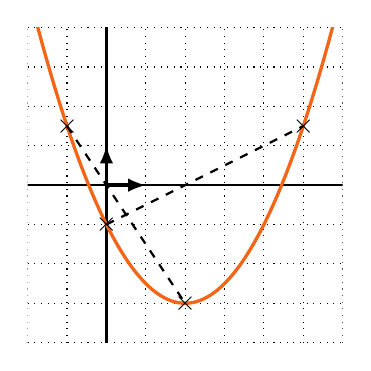
\begin{tikzpicture}[scale=0.5]
\clip (-2,-4) rectangle (6,4);
\draw [ thin, dotted] (-2,-4) grid (6,4);
\draw [thick] (-4,0)--(7,0);
\draw [thick] (0,-4) -- (0,5);
\draw [very thick,->,>=latex] (0,0)--(0,1);
\draw [very thick,->,>=latex] (0,0)--(1,0);
\draw [very thick, ocre,domain=-3:6,samples=100] plot (\x,{\x*\x/2-2*\x-1});
\draw [thick, dashed] (0,-1) -- (5,1.5);
\draw (0,-1) node {$\times$};
\draw (5,1.5) node {$\times$};
\draw [thick, dashed] (-1,1.5) -- (2,-3);
\draw (2,-3) node {$\times$};
\draw (-1,1.5) node {$\times$};
\end{tikzpicture}
\end{center}
\end{minipage}\hfill \begin{minipage}{0.45\linewidth}
\begin{center}
\textbf{Fonction concave}
\end{center}
\begin{center}
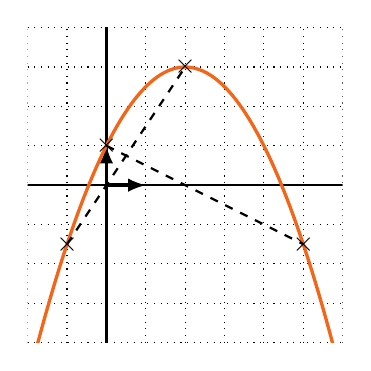
\begin{tikzpicture}[scale=0.5]
\clip (-2,-4) rectangle (6,4);
\draw [thin, dotted] (-2,-4) grid (6,4);
\draw [thick] (-4,0)--(7,0);
\draw [thick] (0,-4) -- (0,5);
\draw [very thick,->,>=latex] (0,0)--(0,1);
\draw [very thick,->,>=latex] (0,0)--(1,0);
\draw [very thick, ocre,domain=-3:6,samples=100] plot (\x,{-(\x*\x/2-2*\x-1)});
\draw [thick, dashed] (0,1) -- (5,-1.5);
\draw (0,1) node {$\times$};
\draw (5,-1.5) node {$\times$};
\draw [thick, dashed] (-1,-1.5) -- (2,3);
\draw (2,3) node {$\times$};
\draw (-1,-1.5) node {$\times$};
\end{tikzpicture}
\end{center}
\end{minipage}






\vskip10pt
\textbf{Rappel de certaines courbes représentatives}
\vskip5pt
\begin{minipage}{0.3\linewidth}
\begin{center}
\textbf{$x \mapsto x^2$}
\end{center}
\begin{center}
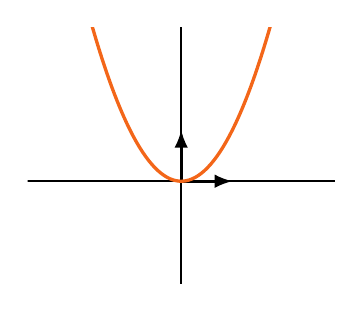
\begin{tikzpicture}[scale=0.65]
\clip (-3,-2) rectangle (3,3);
\draw [thick] (-4,0)--(7,0);
\draw [thick] (0,-4) -- (0,5);
\draw [very thick,->,>=latex] (0,0)--(0,1);
\draw [very thick,->,>=latex] (0,0)--(1,0);
\draw [very thick, ocre,domain=-3:3,samples=100] plot (\x,{\x*\x});
\end{tikzpicture}
\end{center}
\end{minipage}\hfill\begin{minipage}{0.3\linewidth}

\begin{center}
\textbf{$x \mapsto \dfrac{1}{x}$}
\end{center}
\begin{center}
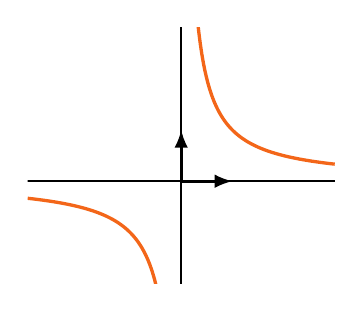
\begin{tikzpicture}[scale=0.65]
\clip (-3,-2) rectangle (3,3);
\draw [thick] (-4,0)--(7,0);
\draw [thick] (0,-4) -- (0,5);
\draw [very thick,->,>=latex] (0,0)--(0,1);
\draw [very thick,->,>=latex] (0,0)--(1,0);
\draw [very thick, ocre,domain=-3:-0.01,samples=100] plot (\x,1/\x);
\draw [very thick, ocre,domain=0.01:3,samples=100] plot (\x,1/\x);
\end{tikzpicture}
\end{center}
\end{minipage}\hfill\begin{minipage}{0.3\linewidth}
\begin{center}
\textbf{$x \mapsto x^3$}
\end{center}
\begin{center}
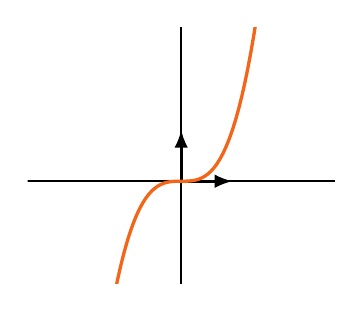
\begin{tikzpicture}[scale=0.65]
\clip (-3,-2) rectangle (3,3);
\draw [thick] (-4,0)--(7,0);
\draw [thick] (0,-4) -- (0,5);
\draw [very thick,->,>=latex] (0,0)--(0,1);
\draw [very thick,->,>=latex] (0,0)--(1,0);
\draw [very thick, ocre,domain=-3:3,samples=100] plot (\x,{\x*\x*\x});
\end{tikzpicture}
\end{center}
\end{minipage}

\begin{minipage}{0.3\linewidth}
\begin{center}
\textbf{$x \mapsto \ln(x)$}
\end{center}
\begin{center}
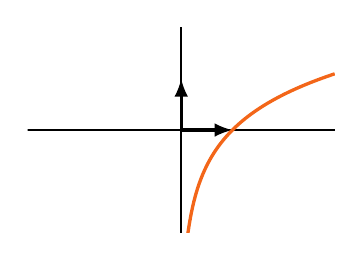
\begin{tikzpicture}[scale=0.65]
\clip (-3,-2) rectangle (3,2);
\draw [thick] (-4,0)--(7,0);
\draw [thick] (0,-4) -- (0,5);
\draw [very thick,->,>=latex] (0,0)--(0,1);
\draw [very thick,->,>=latex] (0,0)--(1,0);
\draw [very thick, ocre,domain=0.1:3,samples=100] plot (\x,{ln(\x)});
\end{tikzpicture}
\end{center}
\end{minipage}
\hfill
\begin{minipage}{0.3\linewidth}
\begin{center}
\textbf{$x \mapsto \e^x$}
\end{center}
\begin{center}
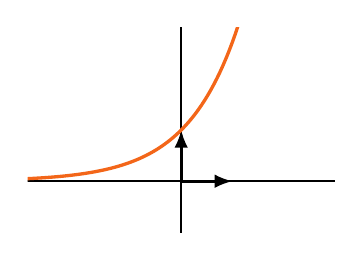
\begin{tikzpicture}[scale=0.65]
\clip (-3,-1) rectangle (3,3);
\draw [thick] (-4,0)--(7,0);
\draw [thick] (0,-4) -- (0,5);
\draw [very thick,->,>=latex] (0,0)--(0,1);
\draw [very thick,->,>=latex] (0,0)--(1,0);
\draw [very thick, ocre,domain=-3:3,samples=100] plot (\x,{exp(\x)});
\end{tikzpicture}
\end{center}
\end{minipage}\hfill
\begin{minipage}{0.3\linewidth}

\begin{center}
\textbf{$x \mapsto \sqrt{x}$}
\end{center}
\begin{center}
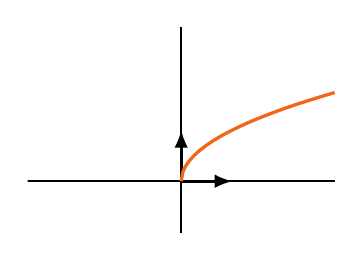
\begin{tikzpicture}[scale=0.65]
\clip (-3,-1) rectangle (3,3);
\draw [thick] (-4,0)--(7,0);
\draw [thick] (0,-4) -- (0,5);
\draw [very thick,->,>=latex] (0,0)--(0,1);
\draw [very thick,->,>=latex] (0,0)--(1,0);
\draw [very thick, ocre,domain=0:3,samples=100] plot (\x,{sqrt(\x)});
\end{tikzpicture}
\end{center}
\end{minipage}

\begin{example} Les fonction $x\mapsto x^2$ et $x\mapsto \e^x$ sont convexes sur $\mathbb{R}$.\\
La fonction $x\mapsto \sqrt{x}$ est concave sur $\mathbb{R}_+$. La fonction $x\mapsto \ln(x)$ est concave sur $\mathbb{R}_+^*$.\\
La fonction $x\mapsto  x^3$ est concave sur $\mathbb{R}_-$ et convexe sur $\mathbb{R}_+$.
\end{example}

\begin{example}Attention : on parle bien de convexité sur un intervalle. Par ailleurs, ce n'est pas parce qu'une fonction $f$ est convexe sur deux intervalles $[a,b]$ et $[b,c]$ que $f$ est aussi convexe sur $[a,c]$.

\begin{center}
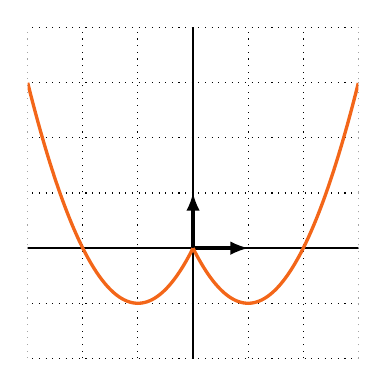
\begin{tikzpicture}[scale=0.7]
\clip (-3,-2) rectangle (3,4);
\draw [ thin, dotted] (-4,-2) grid (4,4);
\draw [thick] (-4,0)--(7,0);
\draw [thick] (0,-4) -- (0,5);
\draw [very thick,->,>=latex] (0,0)--(0,1);
\draw [very thick,->,>=latex] (0,0)--(1,0);
\draw [very thick, ocre,domain=-3:0,samples=100] plot (\x,{(\x+1)^2-1});
\draw [very thick, ocre,domain=0:3,samples=100] plot (\x,{(\x-1)^2-1});
\end{tikzpicture}
\end{center}

La fonction représentée ci-dessus est convexe sur $[-3;0]$ et sur $[0;3]$ mais n'est pas convexe sur $[-3,3]$.\end{example}


\section{Fonctions dérivables}

\subsection{Caractérisation des fonctions convexes}

\begin{proposition}Soit $f$ une fonction définie et dérivable sur un intervalle $I$. On note $\mathcal{C}_f$ la courbe représentative de $f$ dans un repère $\Oij$.
\begin{itemize}
\item $f$ est convexe sur $I$ si et seulement si la courbe $\mathcal{C}_f$ se trouve au-dessus de toutes ses tangentes aux points d'abscisses $x\in I$.
\item $f$ est concave sur $I$ si et seulement si la courbe $\mathcal{C}_f$ se trouve en-dessous de toutes ses tangentes aux points d'abscisses $x\in I$.
\end{itemize}\end{proposition}

\begin{minipage}{0.45\linewidth}
\begin{center}
\textbf{Fonction convexe}
\end{center}
\begin{center}
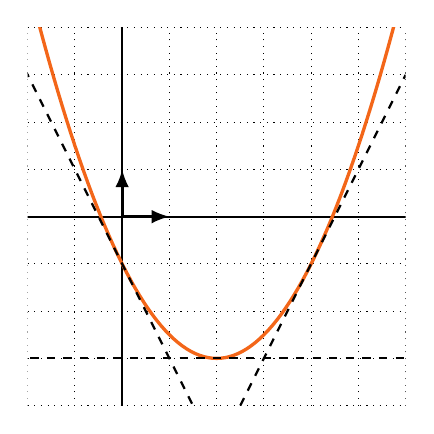
\begin{tikzpicture}[scale=0.6]
\clip (-2,-4) rectangle (6,4);
\draw [ thin, dotted] (-2,-4) grid (6,4);
\draw [thick] (-4,0)--(7,0);
\draw [thick] (0,-4) -- (0,5);
\draw [very thick,->,>=latex] (0,0)--(0,1);
\draw [very thick,->,>=latex] (0,0)--(1,0);
\draw [very thick, ocre,domain=-3:6,samples=100] plot (\x,{\x*\x/2-2*\x-1});
\draw [thick, dashed, domain=-3:6] plot (\x,2*\x-9);
\draw [thick, dashed,domain=-3:6] plot (\x,-3);
\draw [thick, dashed,domain=-3:6] plot (\x,-2*\x-1);

\end{tikzpicture}
\end{center}
\end{minipage}\hfill \begin{minipage}{0.45\linewidth}
\begin{center}
\textbf{Fonction concave}
\end{center}
\begin{center}
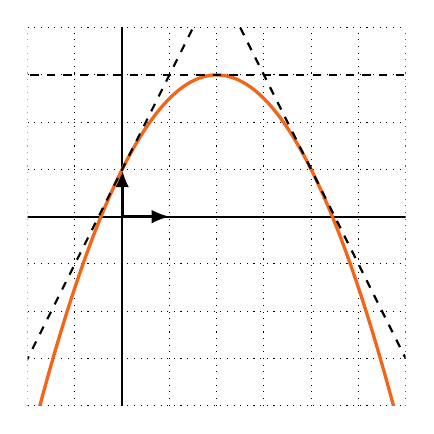
\begin{tikzpicture}[scale=0.6]
\clip (-2,-4) rectangle (6,4);
\draw [thin, dotted] (-2,-4) grid (6,4);
\draw [thick] (-4,0)--(7,0);
\draw [thick] (0,-4) -- (0,5);
\draw [very thick,->,>=latex] (0,0)--(0,1);
\draw [very thick,->,>=latex] (0,0)--(1,0);
\draw [very thick, ocre,domain=-3:6,samples=100] plot (\x,{-(\x*\x/2-2*\x-1)});
\draw [thick, dashed,domain=-3:6] plot (\x,-2*\x+9);
\draw [thick, dashed,domain=-3:6] plot (\x,3);
\draw [thick, dashed,domain=-3:6] plot (\x,2*\x+1);

\end{tikzpicture}
\end{center}
\end{minipage}

\begin{example} Montrons que la fonction $x\mapsto x^2$ est convexe sur $\mathbb{R}$. Notons $\mathcal{C}_f$ la courbe de $f$ dans un repère $(O,\vec i, \vec j)$. Soit $a$ un réel.
\begin{itemize}
\item $f$ est dérivable sur $\mathbb{R}$ et pour tout réel $x$, $f'(x)=2x$.
\item La tangente à $\mathcal{C}_f$ a pour équation $y=f'(a)(x-a)+f(a)$, c'est-à-dire $y=2ax-2a^2+a^2$ ou encore $y=2ax-a^2$.
\item Pour tout réel $x$, 
\[f(x)-(2ax-a^2)=x^2-2ax+a^2=(x-a)^2 \geqslant 0.\]
Ainsi, $\mathcal{C}_f$ est toujours au-dessus de sa tangente à l'abscisse $a$, et ce, peu importe le réel $a$ choisi. $f$ est donc convexe sur $\mathbb{R}$.
\end{itemize}\end{example}




\begin{proposition}Soit $f$ une fonction dérivable sur un intervalle $I$.
\begin{itemize}
\item $f$ est convexe sur $I$ si et seulement si $f'$ est croissante sur $I$.
\item $f$ est concave sur $I$ si et seulement si $f'$ est décroissante sur $I$.
\end{itemize}\end{proposition}

De cette propriété vient naturellement la suivante...

\begin{proposition}Soit $f$ une fonction deux fois dérivable sur un intervalle $I$.
\begin{itemize}
\item $f$ est convexe sur $I$ si et seulement si pour tout $x\in I$, $f''(x) \geqslant 0$.
\item $f$ est concave sur $I$ si et seulement si pour tout $x\in I$, $f''(x) \leqslant 0$. 
\end{itemize}
\end{proposition}

L'étude de la convexité d'une fonction revient à l'étude de signe de sa dérivée seconde (si celle-ci existe, bien entendu).

\begin{demonstration}\textbf{Si $f''\geqslant 0$, alors $f$ est convexe} : Soit $f$ une fonction deux fois dérivable sur $I$ telle que pour tout $x\in I$, $f''(x) \geqslant 0$.

Soit $a\in I$. La tangente à la courbe de $f$ au point d'abscisse $a$ a pour équation $y = f'(a)(x-a)+f(a)$.

Pour tout $x\in I$, posons alors $g(x)=f(x)-(f'(a)(x-a)+f(a))$. $g$ est deux fois dérivable sur $I$, et pour tout $x\in I$, on  $g'(x)=f'(x)-f'(a)$ et $g''(x)=f''(x)$.

Ainsi, puisque pour tout $x\in I$,  $f''(x)\geqslant 0$, on a aussi $g''(x) \geqslant 0$. $g'$ est donc croissante sur $I$. Or, $g'(a)=0$.
Résumons toutes ces informations dans un tableau.

\begin{center}
  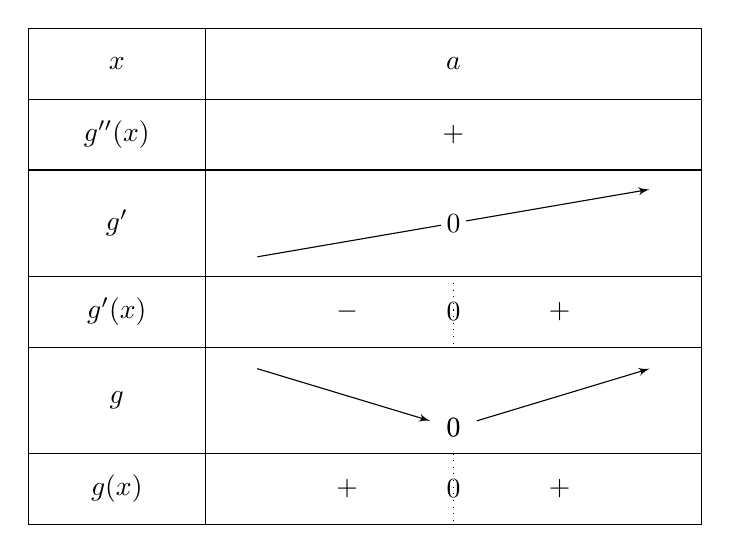
\begin{tikzpicture}[scale=0.9]
  \tikzset{node style/.style = {inner sep = 2pt, outer sep = 2pt}}
   \tkzTabInit[lgt=2.5]{$x$ / 1 , $g''(x)$/1, $g'$/1.5, $g'(x)$/1, $g$/1.5, $g(x)$ / 1}{$ $,$a$,$ $}
	\tkzTabLine{,,+,, }	
   \tkzTabVar{-/$ $,R,+/$ $}
   \tkzTabVal{1}{3}{0.5}{}{$0$}
   \tkzTabLine{,-,z,+ ,}
   \tkzTabVar{+/$ $,-/$0$,+/$ $}
   \tkzTabLine{,+,z,+, }
     
      
   \end{tikzpicture}  
\end{center}

Finalement, pour tout $x\in I$, $g(x)\geqslant 0$, ce qui signifie que $f(x)\geqslant f'(a)(x-a)+f(a)$ : la courbe de $f$ est au-dessus de la tangente à cette courbe au point d'abscisse $a$.\end{demonstration}

\begin{example} Pour tout entier naturel pair $n\geqslant 2$, la fonction $x \mapsto x^n$ est convexe sur $\mathbb{R}$. \\ En effet, la dérivée seconde de cette fonction est la fonction $x\mapsto n(n-1)x^{n-2}$. \\Or, $n$ étant pair, $n-2$ l'est aussi, et pour tout réel $x$, on a donc $x^{n-2}\geqslant 0$.\end{example}

\begin{example}La fonction $f:x\mapsto x^3$ est concave sur $]-\infty ; 0]$ et convexe sur $[0;+\infty[$.

En effet, $f$ est deux fois dérivable sur $\mathbb{R}$ et pour tout réel $x$, $f''(x)=6x$, qui est positif si et seulement si $x$ l'est aussi.\end{example}

\subsection{Point d'inflexion}

\begin{definition}Soit $f$ une fonction dérivable sur un intervalle $I$.

Un \textit{point d'inflexion} est un point où la convexité de la fonction $f$ change. La tangente à la courbe de $f$ en un point d'inflexion traverse la courbe de $f$.\end{definition}

\begin{proposition}Soit $f$ une fonction deux fois dérivable sur un intervalle $I$. 
\begin{itemize}
\item Si $f$ présente un point d'inflexion à l'abscisse $a$, alors $f''(a)=0$.
\item Réciproquement, si $f''(a)=0$ et $f''$ \textbf{change de signe} en $a$, alors $f$ présente un point d'inflexion en $a$.
\end{itemize}\end{proposition}

Cela rappelle naturellement le cas des extremum locaux. Si $f$ admet un extremum local en $a$, alors $f'(a)=0$. Cependant, si $f'(a)=0$, $f$ admet un extremum local en $a$ seulement si $f'$ change de signe en $a$.

\begin{example}Pour tout réel $x$, on pose $f(x)=\dfrac{x^3}{2}-x+1$. 

\begin{minipage}{0.7\linewidth}
$f$ est deux fois dérivable sur $\mathbb{R}$ et pour tout réel $x$, on a $f'(x)=\dfrac{3x^2}{2}-1$ et $f''(x)=3x$.
\vskip5pt
Ainsi, $f''(x) \geqslant 0$ si et seulement si $x\geqslant 0$.
\vskip5pt
$f$ est donc concave sur $]-\infty ;0]$ et convexe sur $[0;+\infty[$.
\vskip5pt
La courbe de $f$ présente un point d'inflexion à l'abscisse 0.
\end{minipage}\hfill\begin{minipage}{0.25\linewidth}
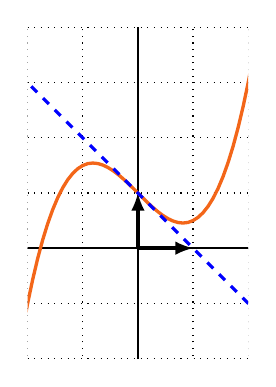
\begin{tikzpicture}[scale=0.7]
\clip (-2,-2) rectangle (2,4);
\draw [thin, dotted] (-2,-4) grid (6,6);
\draw [thick] (-4,0)--(7,0);
\draw [thick] (0,-4) -- (0,6);
\draw [very thick,->,>=latex] (0,0)--(0,1);
\draw [very thick,->,>=latex] (0,0)--(1,0);
\draw [very thick, ocre,domain=-3:6,samples=100] plot (\x,{\x*\x*\x/2-\x+1});
\draw [very thick, blue, dashed,domain=-3:6,samples=100] plot (\x,{1-\x});

\end{tikzpicture}
\end{minipage}

\end{example}

\textbf{Attention : l'annulation de la dérivée seconde n'est pas une condition suffisante de présence d'un point d'inflexion !}


\begin{example}Pour tout réel $x$, on pose $g(x)=\dfrac{1}{12}x^4-\dfrac{2}{3}x^3+2x^2$. 

\begin{minipage}{0.75\linewidth}
La fonction $g$ est deux fois dérivable sur $\mathbb{R}$ et pour tout réel $x$, \\$g'(x)=\dfrac{1}{3}x^3-2x^2+4x$ et $g''(x)=x^2-4x+4=(x-2)^2$.

Ainsi, pour tout réel $x$, $g''(x)\geqslant 0$. $g$ est donc convexe sur $\mathbb{R}$. 

Puisqu'il n'y a pas de changement de convexité, $g$ ne présente pas de point d'inflexion, et ce, même si $g''(2)=0$.
\end{minipage}\hfill\begin{minipage}{0.2\linewidth}
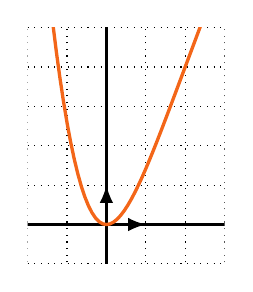
\begin{tikzpicture}[scale=0.5]
\clip (-2,-1) rectangle (3,5);
\draw [thin, dotted] (-2,-4) grid (6,6);
\draw [thick] (-4,0)--(7,0);
\draw [thick] (0,-4) -- (0,6);
\draw [very thick,->,>=latex] (0,0)--(0,1);
\draw [very thick,->,>=latex] (0,0)--(1,0);
\draw [very thick, ocre,domain=-3:6,samples=100] plot (\x,{\x^4/12-2*\x^3/3+2*\x*\x});

\end{tikzpicture}
\end{minipage}

\end{example}

\newpage
\section{Inégalités de convexité}

\subsection{Inégalités de milieux}


\begin{proposition}Soit $f$ une fonction convexe sur un intervalle $I$. 

Pour tous réels $a$ et $b$ de $I$, $ f\left( \dfrac{a+b}{2} \right) \leqslant \dfrac{f(a)+f(b)}{2}$.
\end{proposition}

\begin{demonstration}On considère les points $A(a,f(a))$ et $B(b,f(b))$. 

\begin{minipage}{0.6\linewidth}Le milieu du segment $[AB]$ a pour coordonnées \[\left(\left(\dfrac{a+b}{2}\right),\dfrac{f(a)+f(b)}{2}\right).\] Or, la fonction $f$ étant convexe sur $I$, le segment $[AB]$ se situe au-dessus de la courbe représentative de $f$. En particulier, \[ f\left( \dfrac{a+b}{2} \right) \leqslant \dfrac{f(a)+f(b)}{2}.\]

\end{minipage}\hfill\begin{minipage}{0.35\linewidth}

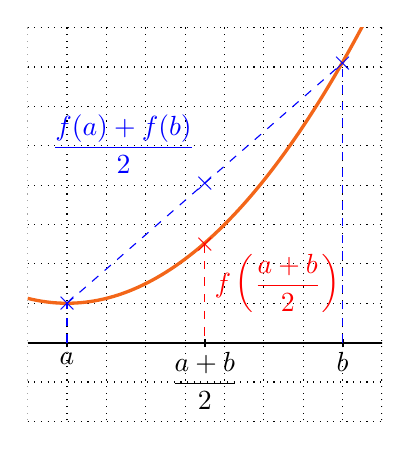
\begin{tikzpicture}[scale=0.5]
\clip (-6,-2) rectangle (3,8);
\draw [thin, dotted] (-6,-4) grid (6,9);
\draw [thick] (-6,0)--(7,0);
\draw [very thick, ocre,domain=-6:6,samples=100] plot (\x,{(\x+5)*(\x+5)/8+1});
\draw [thick] (-5,-0.1) -- (-5,0.1);
\draw (-5,0) node[below] {$a$};
\draw [thick] (2,-0.1) -- (2,0.1);
\draw (2,0) node[below] {$b$};
\draw (-1.5,0) node[below] {$\dfrac{a+b}{2}$};
\draw [thick] (-1.5,-0.1) -- (-1.5,0.1);

\draw [dashed, blue] (2,0) -- (2,7.1);
\draw [dashed, blue] (-5,0) -- (-5,1);
\draw [dashed, blue] (-5,1) -- (2,7.1);
\draw [blue] (2,7.1) node {$\times$};
\draw [blue] (-5,1) node {$\times$};

\draw [blue] (-1.5,4.05) node {$\times$};
\draw [blue] (-1.5,4.05) node[above left] {$\dfrac{f(a)+f(b)}{2}$};

\draw [red] (-1.5,2.5) node {$\times$};
\draw [red,dashed] (-1.5,2.5) -- (-1.5,0);
\draw [red] (-1.5,2.5) node[below right] {$f\left(\dfrac{a+b}{2}\right)$};

\end{tikzpicture}
\end{minipage}

\end{demonstration}

\begin{example}La fonction exponentielle est convexe sur $\mathbb{R}$. Pour tous réels $a$ et $b$, $\exp\left(\dfrac{a+b}{2}\right) \leqslant \dfrac{\e^a+\e^b}{2}$.\end{example}

\begin{proposition}Soit $f$ une fonction concave sur un intervalle $I$. 

Pour tous réels $a$ et $b$ de $I$, $ f\left( \dfrac{a+b}{2} \right) \geqslant \dfrac{f(a)+f(b)}{2}$.
\end{proposition}

\begin{example}La fonction $x\mapsto \sqrt{x}$ est concave sur $\mathbb{R}_+$. 

Ainsi, pour tous réels $a$ et $b$ positifs, $\sqrt{\dfrac{a+b}{2}} \geqslant \dfrac{\sqrt{a}+\sqrt{b}}{2}$.\end{example}

\subsection{Inégalités avec les tangentes}

La convexité des fonctions dérivables permet d'établir des inégalités en utilisant les équations des tangentes.

\begin{example}Montrons que pour tout réel $x$, $\e^x\geqslant x+1$.

\begin{minipage}{0.6\linewidth}
La tangente à la courbe de la fonction exponentielle au point d'abscisse $0$ a pour équation $y=\exp'(0)(x-0)+\exp(0)$, c'est-à-dire $y=x+1$.

Puisque la fonction $\exp$ est convexe sur $\mathbb{R}$, la courbe de la fonction exponentielle est donc au-dessus de toutes ses tangentes et donc, en particulier, la tangente au point d'abscisse 0. On a donc, pour tout réel $x$, $\e^x \geqslant x+1$.

\end{minipage}\hfill\begin{minipage}{0.35\linewidth}

\begin{center}
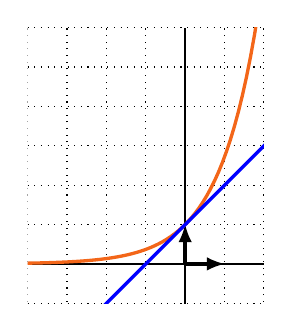
\begin{tikzpicture}[scale=0.5]
\clip (-4,-1) rectangle (2,6);
\draw [thin, dotted] (-4,-4) grid (6,6);
\draw [thick] (-4,0)--(7,0);
\draw [thick] (0,-4) -- (0,6);
\draw [very thick,->,>=latex] (0,0)--(0,1);
\draw [very thick,->,>=latex] (0,0)--(1,0);
\draw [very thick, ocre,domain=-4:6,samples=100] plot (\x,{exp(\x)});
\draw [very thick, blue,domain=-3:6,samples=100] plot (\x,1+\x);
\end{tikzpicture}
\end{center}
\end{minipage}

\end{example}


\chapter{Exercices}

\section*{Convexité}

\begin{exercise}On considère la fonction $f$ dont la courbe représentative est donnée ci-dessous. On a également tracé la tangente à cette courbe au point d'abscisse 0.

\begin{minipage}{0.45\linewidth}
\begin{center}
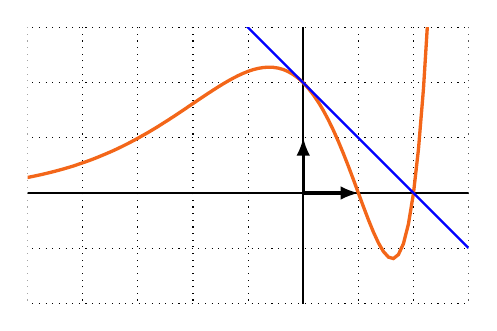
\begin{tikzpicture}[scale=0.7]
\clip (-5,-2) rectangle (3,3);
\draw [ thin, dotted] (-6,-4) grid (6,4);
\draw [thick] (-6,0)--(7,0);
\draw [thick] (0,-4) -- (0,5);
\draw [very thick,->,>=latex] (0,0)--(0,1);
\draw [very thick,->,>=latex] (0,0)--(1,0);
\draw [very thick, ocre,domain=-6:3,samples=100] plot (\x,{(\x*\x-3*\x+2)*exp(\x)});
\draw [thick, blue,domain=-6:3,samples=100] plot (\x,{2-\x});
\end{tikzpicture}
\end{center}\end{minipage}\hfill \begin{minipage}{0.53\linewidth}

\begin{enumerate}
\item Déterminer graphiquement $f'(0)$.
\item Donner une équation réduite de la tangente à la courbe de $f$ au point d'abscisse 0.
\item Déterminer graphiquement le signe de $f'(-3)$.
\item La fonction $f$ semble-t-elle convexe ou concave sur  $[-5\, ;\, -2]$ ? sur $[-2\,;\,1]$ ? sur $[1 \, ; 2\,]$ ?
\end{enumerate}\end{minipage}\end{exercise}


\begin{solution}

\(f'(0)\) est le coefficient directeur de la tangente à la courbe de \(f\) à l'abscisse 0. Ce coefficient directeur vaut \(-1\). Ainsi, \(f'(0)=-1\).

La tangente à la courbe de \(f\) au point d'abscisse 0 a pour coefficient directeur \(-1\) et pour ordonnée à l'origine 2. L'équation réduite de cette tangente est donc \(y=-x+2\).
 
\(f\) est dérivable et croissante sur \([2;4]\). Ainsi, pour tout réel \(x \in [2;4]\), \(f'(x)\geqslant 0\). En particulier, \(f'(3)\geqslant 0\).

La fonction \(f\) semble convexe \([-5\, ;\, -2]\), concave sur \([-2\,;\,1]\) et convexe sur \([1 \, ; 2\,]\).
\end{solution}



\begin{exercise}On considère une fonction $f$ dont le tableau de variations est donné ci-dessous.
\begin{center}
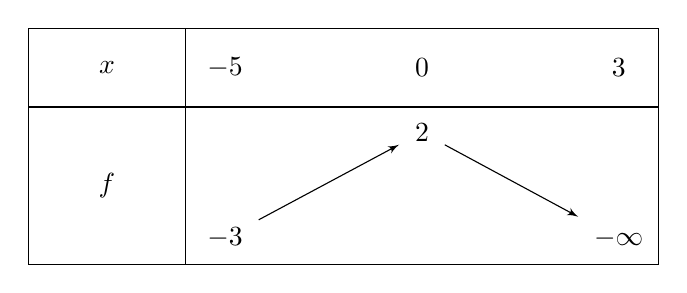
\begin{tikzpicture}[scale=1]
   \tkzTabInit[espcl=2.5]{$x$ / 1, $f$/2}{$-5$, $0$ ,$3$}
      \tkzTabVar{ -/$-3$, +/$2$, -/$-\infty$}
\end{tikzpicture}
\end{center}

On sait de plus que $f$ est convexe sur $[-5;-2]$ puis concave sur $[-2;3]$. Tracer une courbe représentative compatible avec ces données.\end{exercise}

\begin{solution}La fonction suivante convient : 

\begin{center}
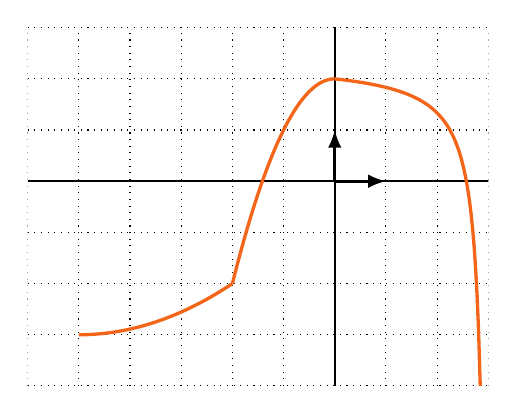
\begin{tikzpicture}[scale=0.65]
\clip (-6,-4) rectangle (3,3);
\draw [ thin, dotted] (-6,-4) grid (6,4);
\draw [thick] (-6,0)--(7,0);
\draw [thick] (0,-4) -- (0,5);
\draw [very thick,->,>=latex] (0,0)--(0,1);
\draw [very thick,->,>=latex] (0,0)--(1,0);
\draw [very thick, ocre,domain=0:2.9,samples=100] plot (\x,{(1/(\x-3)+7/3});
\draw [very thick, ocre,domain=-2:0,samples=100] plot (\x,{2-\x*\x});
\draw [very thick, ocre,domain=-5:-2,samples=100] plot (\x,{\x*\x/9  + 10* \x/9-2/9 });
\end{tikzpicture}
\end{center}
\end{solution}




\begin{exercise}L'objectif de cet exercice est de démontrer que la fonction $x\mapsto x^2$ est convexe sur $\mathbb{R}$. Le plan est muni d'un repère orthonormé $\Oij$. On note $\mathcal{C}$ la courbe de la fonction $x\mapsto x^2$ dans ce repère.
\begin{enumerate}
\item \textbf{Cas particulier} : On considère les points $A$ et $B$ de coordonnées respectives $(-2;4)$ et $(3;9)$.
\begin{enumerate}
\item Justifier que ces points appartiennent bien à la courbe $\mathcal{C}$.
\item Vérifier que l'équation réduite de la droite $(AB)$ est $y=x+6$.
\item Étudier le signe de $x^2-(x+6)$ sur l'intervalle $[-2;3]$ et conclure.
\end{enumerate}
\item \textbf{Cas général} Soit $a$ et $b$ deux réels avec $a<b$, $A(a\,,\,a^2)$ et $B(b\,,\,b^2)$ deux points de la courbe $\mathcal{C}$.
\begin{enumerate}
\item Montrer que l'équation réduite de la droite $(AB)$ est $y=(a+b)x-ab$.
\item Étudier le signe de $x^2-((a+b)x-ab)$ sur $[a;b]$ et conclure.
\end{enumerate}
\end{enumerate}\end{exercise}

\begin{solution}\hspace{0pt}
\begin{enumerate}\item \begin{enumerate}\item Puisque \((-2)^2=4\) et que \(3^2=9\), les points \(A\) et \(B\) appartiennent bien à la courbe \(\mathcal{C}\).
	\item Le coefficient directeur de la droite \((AB)\) vaut \(\dfrac{9-4}{3-(-2)}\), c'est-à-dire 1. L'équation réduite de la droite \((AB)\) est donc de la forme \(y=x+p\). Par ailleurs, le point \(A\) appartient à cette droite, ses coordonnées en vérifient donc l'équation. Ainsi, \(4=-2+p\) et donc \(p=6\). L'équation réduite de la droite \((AB)\) est \(y=x+6\).
	\item \(x^2-(x+6)\) est un polynôme du second degré dont les racines sont \(-2\) et \(3\) (ce sont les abscisses des points \(A\) et \(B\), qui sont les points d'intersection de la courbe de \(f\) et de la droite \((AB)\)). Ainsi, \(x^2-(x+6)\) est négatif pour \(x \in [-2;3]\), ce qui signifie que sur cet intervalle, \(x^2 \leqslant x+6\) : la courbe de la fonction \(f\) se situe sous la droite \((AB)\).\end{enumerate}
	
	\item \begin{enumerate}\item Le coefficient directeur de la droite \((AB)\) vaut \(\dfrac{b^2-a^2}{b-a}=\dfrac{(b-a)(b+a)}{b-a}=a+b\). L'équation réduite de la droite \((AB)\) est donc de la forme \(y=(a+b)x+p\). Par ailleurs, le point \(A\) appartient à cette droite, ses coordonnées en vérifient donc l'équation. Ainsi, \(a^2=(a+b)a+p\) et donc \(p=a^2-a(a+b)=-ab\). L'équation réduite de la droite \((AB)\) est \(y=(a+b)x-ab\).
	\item \(x^2-((a+b)x-ab)\) est un polynôme du second degré dont les racines sont \(a\) et \(b\) (ce sont les abscisses des points \(A\) et \(B\), qui sont les points d'intersection de la courbe de \(f\) et de\((AB)\)). \\ Ces racines peuvent par ailleurs se trouver en utilisant les relations entre coefficients et racines. Ainsi, \(x^2-((a+b)x-ab)\) est négatif pour \(x \in [a;b]\), ce qui signifie que sur cet intervalle, \(x^2 \leqslant (a+b)x-ab\) : la courbe de la fonction \(f\) se situe sous la droite \((AB)\). Ceci valant peu importe les valeurs de \(a\) et \(b\), on trouve bien que la fonction \(f\) est convexe sur \(\mathbb{R}\).\end{enumerate}\end{enumerate}
\end{solution}


\begin{exercise}En vous inspirant du cas général de l'exercice précédent, montrer que la fonction $x\mapsto \dfrac{1}{x}$ est convexe sur $]0;+\infty[$.\end{exercise}

\begin{solution}Soit $a$ et $b$ deux réels tels que $0<a<b$. On considère les points $A\left(a;\dfrac{1}{a}\right)$ et $B\left(b;\dfrac{1}{b}\right)$. Ces points se trouvent sur la courbe de la fonction inverse.

Le coefficient directeur de la droite \((AB)\) vaut \(\dfrac{\frac{1}{b}-\frac{1}{a}}{b-a}\), c'est-à-dire \(\dfrac{(a-b)(ab)}{b-a}\) et donc vaut \(-\dfrac{1}{ab}\). L'équation réduite de la droite \((AB)\) est donc de la forme \(y=-\dfrac{1}{ab}x+p\). Par ailleurs, le point \(A\) appartient à cette droite, ses coordonnées en vérifient donc l'équation. Ainsi, \(\dfrac{1}{a}=-\dfrac{a}{ab}+p\) et donc \(p=\dfrac{1}{a}+\dfrac{1}{b}\). L'équation réduite de la droite \((AB)\) est \(y=-\dfrac{1}{ab}x+\dfrac{1}{a}+\dfrac{1}{b}\).

Soit donc $x\in [a;b]$. On a
\[\dfrac{1}{x}-\left(-\dfrac{1}{ab}x+\dfrac{1}{a}+\dfrac{1}{b}\right)=\dfrac{ab}{xab}+\dfrac{x^2}{xab}-\dfrac{bx}{xab}-\dfrac{ax}{xab}=\dfrac{x^2-(a+b)x+ab}{xab}\]
Or, $xab>0$. De plus, \(x^2-((a+b)x-ab)\) est un polynôme du second degré dont les racines sont \(a\) et \(b\) (ce sont les abscisses des points \(A\) et \(B\), qui sont les points d'intersection de la courbe de la fonction inverse et de la droite \((AB)\)). Ces racines peuvent par ailleurs se trouver en utilisant les relations entre coefficients et racines. Ainsi, \(x^2-((a+b)x-ab)\) est négatif pour \(x \in [a;b]\). On a donc \(\dfrac{1}{x} \leqslant -\dfrac{1}{ab}x+\dfrac{1}{a}+\dfrac{1}{b}\) : la courbe de la fonction inverse se situe sous la droite $(AB)$, peu importe les valeurs de $a$ et $b$. La fonction inverse est donc convexe sur $]0;+\infty[$.
\end{solution}




\section*{Convexité des fonctions dérivables}

\begin{exercise}On considère la fonction $f:x\mapsto \dfrac{1}{x}$, définie et dérivable sur $]0;+\infty[$. Soit $a>0$.
\begin{enumerate}
\item Montrer que pour tout réel strictement positif $x$, 
\[f(x)-(f'(a)(x-a)+f(a))=\dfrac{(a-x)^2}{a^2x}.\]
\item La fonction $f$ est-elle convexe ou concave sur $]0;+\infty[$ ?
\end{enumerate}\end{exercise}

\begin{solution}
Pour tout réel strictement positif \(x\),
\[f(x)-(f'(a)(x-a)+f(a))  = \dfrac{1}{x} - \left( -\dfrac{1}{a^2}(x-a)+\dfrac{1}{a}\right) = \dfrac{1}{x}+ \dfrac{x}{a^2} - \dfrac{1}{a} -\dfrac{1}{a}\]
d'où 
\[f(x)-(f'(a)(x-a)+f(a)) = \dfrac{1}{x} + \dfrac{x}{a^2}-\dfrac{2}{a} =\dfrac{a^2}{xa^2}+\dfrac{x^2}{xa^2} - \dfrac{2ax}{xa^2} = \dfrac{a^2-2ax+x^2}{xa^2}= \dfrac{(a-x)^2}{xa^2} .\]

Or, puisque \(x > 0\), cette quantité est positive. Il en vient que pour tout \(x>0\), \(f(x)-(f'(a)(x-a)+f(a)) \geqslant 0\) et donc que \(f(x)\geqslant (f'(a)(x-a)+f(a) \). Cela se traduit par le fait que sur \(]0;+\infty[\), la courbe de la fonction inverse est au-dessus de toutes ses tangentes : cette fonction est donc convexe sur \(]0;+\infty[\).\end{solution}

\begin{exercise}[subtitle={(Polynésie 2022)}]

On considère une fonction $f$ définie et dérivable sur $|-2;2]$. Le tableau de variations de la fonction $f'$, dérivée de la fonction $f$ sur l'intervalle $[-2;2]$ est donné par :
\begin{center}
  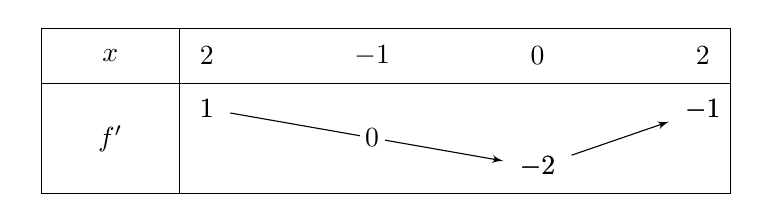
\begin{tikzpicture}[scale=0.7]
  \tikzset{node style/.style = {inner sep = 2pt, outer sep = 2pt}}
   \tkzTabInit[lgt=2.5]{$x$ / 1 , $f'$ / 2}{$2$,$-1$,$0$,$2$}

   \tkzTabVar{+/$1$,R,-/$-2$,+/$-1$}
   \tkzTabIma{1}{3}{2}{0}
     
      
   \end{tikzpicture}  
\end{center}

Parmi les affirmations suivantes, laquelle est exacte ?

\begin{tabularx}{\linewidth}{XX}
\textbf{a.} $f$ est convexe sur $[-2;-1]$. & \textbf{b.} $f$ est concave sur $[0;1]$. \\
\textbf{c.} $f$ est convexe sur $[-1;2]$. & \textbf{d.} $f$ est concave sur $[-2;0]$.
\end{tabularx}\end{exercise}

\begin{solution}Attention à bien remarquer qu'il s'agit des variations de la dérivée ! La fonction $f'$ est décroissante sur $[-2;0]$. $f$ est donc concave sur cet intervalle.\end{solution}



\begin{exercise}On donne la représentation graphique de la \textbf{fonction dérivée} $f'$ d'une fonction $f$ définie sur $\mathbb{R}$. 

\begin{minipage}{0.6\linewidth}
Parmi les affirmations suivantes, laquelle est correcte ?
\begin{itemize}
\item $f$ est concave sur $]0;+\infty[$.
\item $f$ est convexe sur $]0;+\infty[$.
\item $f$ est convexe sur $[0;2]$.
\item $f$ est convexe sur $[2;+\infty[$.
\end{itemize}
\end{minipage}\hfill\begin{minipage}{0.35\linewidth}
\begin{center}
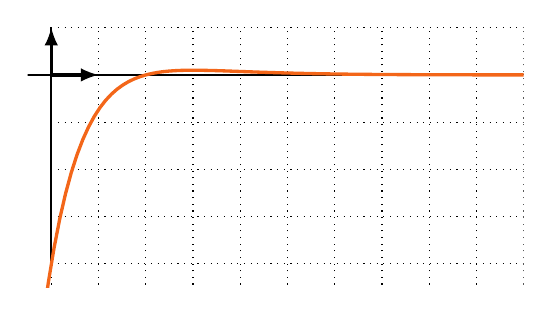
\begin{tikzpicture}[scale=0.6]
\clip (-0.5,-4.5) rectangle (10,1);
\draw [ thin, dotted] (0,-5) grid (10,1);
\draw [thick] (-6,0)--(7,0);
\draw [thick] (0,-4) -- (0,5);
\draw [very thick,->,>=latex] (0,0)--(0,1);
\draw [very thick,->,>=latex] (0,0)--(1,0);
\draw [very thick, ocre,domain=-2:10,samples=100] plot (\x,{2*(\x-2)*exp(-\x)});

\end{tikzpicture}
\end{center}
\end{minipage}
\end{exercise}

\begin{solution}Attention à bien remarquer qu'il s'agit là de la représentation graphique de la dérivée ! La fonction $f'$ est croissante sur $[0;2]$, $f$ est donc convexe sur cet intervalle.\end{solution}




\begin{exercise}Soit $a$ et $b$ deux réels. Montrer que la fonction $x\mapsto \e^{ax+b}$, définie et deux fois dérivable sur $\mathbb{R}$,  est également convexe sur $\mathbb{R}$.\end{exercise}

\begin{solution}La fonction  \(f:x\mapsto \e^{ax+b}\) est deux fois dérivable sur \(\mathbb{R}\). De plus, pour tout réel \(x\), \(f'(x)=a\e^{ax+b}\) et \(f^{\prime\prime}(x)=a^2\e^{ax+b}\geqslant 0\). Cette fonction est donc convexe sur \(\mathbb{R}\).\end{solution}


\begin{exercise}Montrer que la fonction $\ln$ est concave sur $]0;+\infty[$.\end{exercise}

\begin{solution}La fonction \(\ln\) est dérivable sur \(]0;+\infty[\) et, pour tout réel \(x>0\), \(\ln '(x)=\dfrac{1}{x}\) et \(\ln^{\prime\prime}(x)=-\dfrac{1}{x^2}\leqslant 0\). Il en vient que la fonction \(\ln\) est concave sur \(]0;+\infty[\).\end{solution}



\begin{exercise}Pour tout réel $x$, on pose $f(x)=3x^3+3x^2-4x+1$
\begin{enumerate}
\item Pour tout réel $x$, déterminer $f''(x)$.
\item En déduire les intervalles sur lesquels $f$ est convexe.
\item La fonction $f$ possède-t-elle un point d'inflexion ? Si oui, en quelle abscisse ?
\end{enumerate}\end{exercise}

\begin{solution}
Pour tout réel \(x\), \(f'(x)=9x^2+6x-4\) et \(f^{\prime\prime}(x)=18x+6\).

On a \(f^{\prime\prime}(x)\geqslant 0\) si et seulement si \(x \geqslant - \dfrac{1}{3}\). \(f\) est donc convexe sur \(\left]-\dfrac{1}{3};+\infty\right[\).

La convexité de \(f\) change à l'abscisse \(-\dfrac{1}{3}\). La courbe de \(f\) présente donc un point d'inflexion à cette abscisse.\end{solution}



\begin{exercise}Pour tout réel $x$, on pose $f(x)=x^4+2x^2-3x+1$. La fonction $f$ admet-elle un point d'inflexion ?\newpage \end{exercise}

\begin{solution}
\(f\) est deux fois dérivables sur \(\mathbb{R}\) et pour tout réel \(x\), \(f^{\prime\prime}(x)=12x^2+4\) qui est strictement positif. La fonction \(f\) est convexe sur \(\mathbb{R}\). Sa convexité ne change pas, la courbe de \(f\) ne possède donc pas de point d'inflexion.\end{solution}



\begin{exercise}Soit $a$, $b$, $c$ et $d$ des réels avec $a \neq 0$. Montrer que la fonction $f:x\mapsto ax^3+bx^2+cx+d$ admet un point d'inflexion.\end{exercise}

\begin{solution}$f$ est deux fois dérivable sur $\mathbb{R}$ et pour tout réel $x$, $f'(x)=3ax^2+2bx+c$ et $f''(x)=6ax+2b$. Ainsi, $f''$ change de signe en $-\dfrac{b}{3a}$. $f$ admet donc un point d'inflexion.\end{solution}



\begin{exercise}On considère la fonction $f:x\mapsto \ln(1+x^2)$.
\begin{enumerate}
\item Justifier que $f$ est définie et dérivable sur $\mathbb{R}$ et calculer $f'(x)$.
\item Construire le tableau de variations de $f$ en y incluant les limites.
\item Résoudre l'équation $f(x)=1$ sur $\mathbb{R}$.
\item Justifier que $f$ est deux fois dérivable sur $\mathbb{R}$ et que pour tout réel $x$
\[ f''(x)= \dfrac{2-2x^2}{(1+x^2)^2}.\]
\item Construire le tableau de signes de $f''$ et en déduire les intervalles lesquels $f$ est convexe/concave.
\item Donner les équations des tangentes à la courbe de $f$ aux points d'abscisses 1 et $-1$.
\item Dans un repère orthonormé, tracer la courbe représentative de $f$ ainsi que ses tangentes aux points d'abscisse 1 et $-1$.
\end{enumerate}\end{exercise}

\begin{solution}\hspace{0pt}
\begin{enumerate}\item La fonction \(u:x\mapsto 1+x^2\) est dérivable et strictement positive sur \(\mathbb{R}\). Or $f=\ln(u)$. \(f\) est donc dérivable sur $\mathbb{R}$ et $f'=\dfrac{u'}{u}$ : pour tout \(x\in\mathbb{R}\), $f'(x)=\dfrac{2x}{1+x^2}$.
\item 
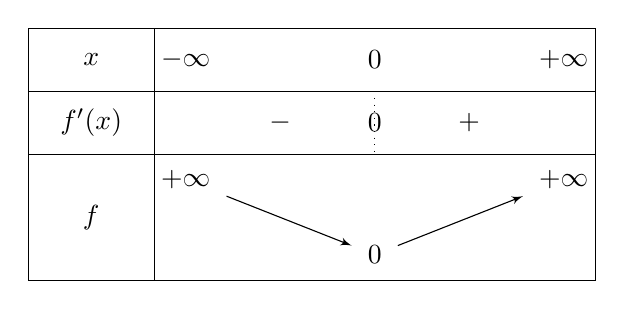
\begin{tikzpicture}[scale=0.8]
   \tkzTabInit{$x$ / 1 , $f'(x)$ / 1, $f$ / 2}{$-\infty$, $0$, $+\infty$}
   \tkzTabLine{,-,z,+, }
   \tkzTabVar{+/$+\infty$,-/$0$,+/$+\infty$}
\end{tikzpicture}


\item Soit \(x\) un réel,
	\[f(x)=1 \Leftrightarrow \ln(1+x^2)=1 \Leftrightarrow 1+x^2=e \Leftrightarrow x^2=e-1 \Leftrightarrow x=\sqrt{e-1} \text{ ou }x = -\sqrt{e-1}.\]
	\item \(f'\) est dérivable comme produit de deux fonctions dérivables dont le dénominateur ne s'annule pas. Pour tout réel \(x\),
\[f^{\prime\prime}(x)= \dfrac{2(1+x^2)-2x \times 2x}{(1+x^2)^2}=\dfrac{2-2x^2}{(1+x^2)2}.\]
Or, \(f^{\prime\prime}(x)\geqslant 0\) si et seulement si \(x \in [-1;1]\). \(f\) est donc convexe sur \([-1;1]\) et concave sur \(]-\infty;-1]\) et \([1;+\infty[\).
\item La tangente à la courbe de\(f\) à l'abscisse \(-1\) a pour équation réduite \[y = f'(-1)(x+1)+f(-1) = -(x+1)+\ln(2)=-x+\ln(2)-1.\]
	La tangente à la courbe de\(f\) à l'abscisse \(1\) a pour équation réduite \[y = f'(1)(x-1)+f(1) = x-1+\ln(2).\]
	\item On trace la courbe de $f$ dans un repère orthonormé.
\begin{center}
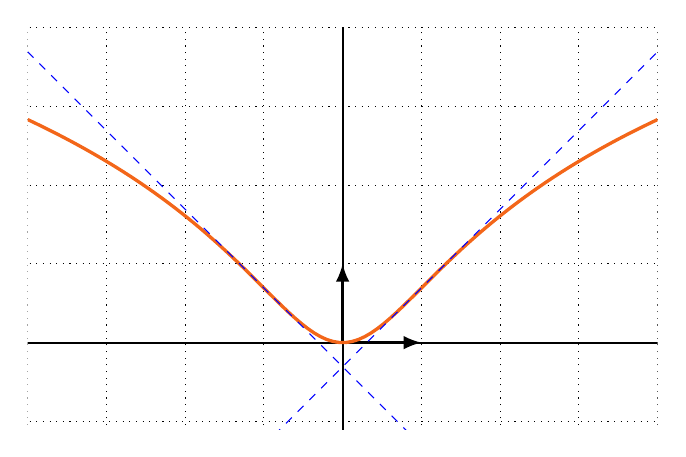
\begin{tikzpicture}[scale=1]
\clip (-4,-1.1) rectangle (4,4);
\draw [ thin, dotted] (-6,-4) grid (6,4);
\draw [thick] (-6,0)--(7,0);
\draw [thick] (0,-4) -- (0,5);
\draw [very thick,->,>=latex] (0,0)--(0,1);
\draw [very thick,->,>=latex] (0,0)--(1,0);
\draw [very thick, ocre,domain=-4:4,samples=100] plot (\x,{ln(1+\x*\x)});
\draw [blue, dashed,domain=-4:4,samples=100] plot (\x,{\x + ln(2)-1});
\draw [blue, dashed,domain=-4:4,samples=100] plot (\x,{-\x + ln(2)-1});
\end{tikzpicture}
\end{center}
\end{enumerate}
\end{solution}




\begin{exercise}On considère la fonction définie pour tout réel $x$ par $f(x)=\dfrac{1}{1+\e^{-x}}$.
\begin{enumerate}
\item Justifier que pour tout réel $x$, $0<f(x)<1$.
\item Déterminer $\displaystyle \lim _{x \to +\infty}f(x)$ et $\displaystyle \lim _{x \to -\infty}f(x)$.
\item Montrer que $f$ est strictement croissante sur $\mathbb{R}$.
\item Résoudre l'équation $f(x)=\dfrac{3}{4}$ sur $\mathbb{R}$.
\item Justifier que $f$ est deux fois dérivable sur $\mathbb{R}$ et montrer que pour tout réel $x$,
\[f''(x) = \dfrac{\e^{-x}(\e^{-x}-1)}{(1+\e^{-x})^3}.\]
\item En déduire les intervalles sur lesquels $f$ est convexe/concave.
\end{enumerate}\end{exercise}

\begin{solution}\hspace{0pt} 
\begin{enumerate}
\item D'une part, pour tout réel $x$, $1+\e^{-x}>0$. Il en vient que $f(x)>0$ comme quotient de deux nombres strictement positifs. Par ailleurs, pour tout réel $x$, $1+\e^{-x}>1$, et donc, par stricte décroissance de la fonction inverse sur $]0;+\infty[$, on a $\dfrac{1}{1+\e^{-x}}<1$.
\item On a $\displaystyle\lim_{x\to+\infty}\e^{-x}=0$ et $\displaystyle\lim_{x\to -\infty}f(x)=+\infty$. En utilisant les règles d'opération sur les limites, on en conclut que $\displaystyle\lim_{x\to +\infty}f(x)=1$ et $\displaystyle\lim_{x\to -\infty}f(x)=0$.
\item $f$ est dérivable sur $\mathbb{R}$ et pour tout réel $x$, $f'(x)=-\dfrac{-\e^{-x}}{(1+\e^{-x})^2}=\dfrac{\e^{-x}}{(1+\e^{-x})^2}>0$. $f$ est donc croissante sur $\mathbb{R}$.
\item Soit $x\in\mathbb{R}$.
\[f(x)=\dfrac{3}{4}\Leftrightarrow \dfrac{1}{1+\e^{-x}} = \dfrac{3}{4} \Leftrightarrow 3+3\e^{-x} = 4 \Leftrightarrow \e^{-x}=\dfrac{1}{3} \Leftrightarrow -x=\ln(\left(\dfrac{1}{3}\right) \Leftrightarrow x = -\ln\left(\dfrac{1}{3}\right)=\ln(3).\]
\item $f'$ est dérivable sur $\mathbb{R}$ comme quotient de fonctions dérivables dont le dénominateur ne s'annule pas. Pour tout réel $x$, on pose $u(x)=(1+\e^{-x})^2$. On a alors, pour tout réel $x$, $u'(x)=2 \times (-\e^{-x}) \times (1+\e^{-x})$. Ainsi, pour tout réel $x$,
\[f''(x)=\dfrac{-\e^{-x}(1+\e^{-x})^2-\e^{-x}\times(-2\e^{-x}(1+\e^{-x}))}{(1+\e^{-x})^4}=\dfrac{\e^{-x}(1+\e^{-x})(-(1+\e^{-x})+2\e^{-x})}{(1+\e^{-x})^4}\]
et donc 
\[f''(x)=\dfrac{\e^{-x}(\e^{-x}-1)}{(1+\e^{-x})^3}.\]
\item Pour tout réel $x$, $\e^{-x}>0$ et $(1+\e^{-x})^3>0$. Ainsi, $f''(x)$ est du signe de $\e^{-x}-1$. Or, $\e^{-x}-1\geqslant 0$ si et seulement si $\e^{-x}\geqslant 1$ soit $-x\geqslant 0$ et donc $x\leqslant 0$. Ainsi, $f$ est convexe sur $]-\infty;0]$ et concave sur $[+;+\infty[$.
\end{enumerate}\end{solution}



\begin{exercise}[subtitle={(Amérique du Nord 2022)}]Vrai ou faux ? On considère la fonction h définie sur $\mathbb{R}$ par  $h(x) = \e^x(1-x^2)$. Dans le plan muni d'un repère orthonormé, la courbe représentative de la fonction $h$ n'admet pas de point d'inflexion.\end{exercise}

\begin{solution}$f$ est deux fois dérivable sur $\mathbb{R}$ et pour tout réel $x$, $h'(x)=\e^x(1-x^2)+\e^x(-2x)=\e^x(1-2x-x^2)$ puis $h''(x)=\e^x(1-2x-x^2)+\e^x(-2-2x)=\e^x(-1-4x-x^2)=-\e^x(x^2+4x+1)$. Pour tout réel $x$, $\e^x>0$. Par ailleurs, $x^2+4x+1$ est un polynôme du second degré dont le discriminant vaut $12$. Il admet donc deux racines réelles qui correspond aux changements de signes du polynôme $x^2+4x+1$. En particulier, la courbe de $h$ admet deux points d'inflexion.\end{solution}



\begin{exercise}Soit $f$ une fonction dérivable, convexe et croissante sur un intervalle $[a;+\infty[$. \\Montrer que $\displaystyle\lim_{x \to + \infty}f(x)=+\infty$.\newpage \end{exercise}

\begin{solution}
Puisque \(f\) est dérivable est strictement croissante sur \([a;+\infty[\), il existe donc un réel \(c\) dans cet intervalle tel que \(f'(c)>0\).

 Or, \(f\) est convexe sur \([a;+\infty[\), la courbe de \(f\) est donc au-dessus de ses tangentes sur cet intervalle, et en particulier au-dessus de la tangente en \(c\). 

 Une équation réduite de cette tangente est de la forme \(y = f'(c)x -cf'(c)+f(c)\). 

 Ainsi, pour tout \(x \in [a;+\infty[\), on a \(f(x) \geqslant f'(c)x -cf'(c)+f(c)\). \\Or, \(\displaystyle\lim_{x\to +\infty}(f'(c)x -cf'(c)+f(c))=+\infty\), et il en vient que, par comparaison, \(\displaystyle\lim_{x \to + \infty}f(x)=+\infty\).\end{solution}
 
 

 
\section*{Inégalités de convexité}

\begin{exercise}On considère la fonction $f:x\mapsto \sqrt{x}$, définie sur $[0;+\infty [$.
\begin{enumerate}
\item Pour tout réel $x>0$, déterminer une expression de $f'(x)$ et de $f''(x)$.
\item $f$ est-elle convexe ou concave sur $]0;+\infty[$ ?
\item Déterminer l'équation de la tangente à la courbe de $f$ au point d'abscisse 1.
\item En déduire que pour tout réel $x>0$, $\sqrt{x} \leqslant \dfrac{x}{2}+\dfrac{1}{2}$. Représenter graphiquement cette inégalité.
\end{enumerate}\end{exercise}

\begin{solution}
\(f\) est deux fois dérivable sur \(]0;+\infty [\).

Pour tout réel \(x>0\), \(f'(x)=\dfrac{1}{\sqrt{x}}\) et $f^{\prime\prime}(x)=\dfrac{-\frac{1}{2\sqrt{x}}}{\sqrt{x}^2}=-\dfrac{1}{2x\sqrt{x}}$.

Puisque pour tout \(x>0\), \(f^{\prime\prime}(x)\leqslant 0\), \(f\) est concave sur \(]0;+\infty[\).

L'équation de la tangente à la courbe de \(f\) au point d'abscisse 1 est
\[ y=f'(1)(x-1)+f(1)=\dfrac{1}{2}(x-1)+1\quad\text{soit}\quad y=\dfrac{x}{2}+\dfrac{1}{2}.\]

 Puisque \(f\) est concave, elle est sous toutes ses tangentes. Ainsi, pour tout réel \(x>0\), \(\sqrt{x} \leqslant \dfrac{x}{2}+\dfrac{1}{2}\).
\end{solution}




\begin{exercise}Soit $n$ un entier naturel non nul. On considère la fonction $f:x\mapsto (1+x)^n$.
\begin{enumerate}
\item La fonction $f$ est-elle convexe ou concave sur $[0;+\infty[$ ?
\item En utilisant la tangente à la courbe de $f$ au point d'abscisse 0, montrer que pour tout réel $x\geqslant 0$,  on a $(1+x)^n \geqslant 1+nx$.
\item Quelle inégalité a-t-on redémontré ?
\end{enumerate}\end{exercise}

\begin{solution}\(f\) est deux fois dérivable sur \([0;+\infty[\) et pour tout réel \(x\geqslant 0\), \(f'(x)=n(1+x)^{n-1}\) et \\ \(f^{\prime\prime}(x)=n(n-1)(1+x)^{n-2}\). Puisque $x\geqslant 0$, alors \(f^{\prime\prime}(x) \geqslant 0\) et \(f\) est donc convexe sur \([0;+\infty[\).

De plus, la tangente à l'abscisse 0 à la courbe de \(f\) a pour équation \(y=f'(0)(x-0)+f(0)\) soit \(y=1+nx\).

\(f\) étant convexe sur \([0;+\infty[\), sa courbe se trouve au-dessus de toutes ses tangente sur cet intervalle. En particulier, pour tout réel \(x\geqslant 0\), 
\[(1+x)^n \geqslant 1+nx .\]

On retrouve ici l'inégalité de Bernoulli.\end{solution}



\begin{exercise}En utilisant la tangente à la courbe de la fonction $\ln$ en 1, montrer que pour tout $x>0$, $\ln(x) \leqslant x -1$.\end{exercise}

\begin{solution}
La tangente à la courbe du logarithme népérien à l'abscisse 1 a pour équation
\[ y =\ln'(1)(x-1)+\ln(1)=x-1.\]
Le logarithme népérien est concave : sa dérivée seconde est la fonction \(x\mapsto -\dfrac{1}{x^2}\) qui est négative sur \(]0;+\infty[\). Ainsi, la courbe représentative de la fonction \(\ln\) se situe sous ses tangentes.

En particulier, pour tout réel \(x\), \(\ln(x) \leqslant x-1\).\end{solution}



\begin{exercise}On considère la fonction $f$ définie sur $]0;+\infty[$ par $f(x)=(\ln(x))^2$.
\begin{enumerate}
\item Déterminer les intervalles sur lesquels $f$ est convexe/concave.
\item En utilisant une équation de la tangente à la courbe représentative de $f$ au point d'abscisse $e$, montrer que pour tout réel $x$ dans $]0;e]$,
\[(\ln(x))^2\geqslant \dfrac{2}{e}x-1.\]
\end{enumerate}\end{exercise}

\begin{solution}
$f$ est deux fois dérivable sur $]0;+\infty[$ et pour tout réel $x>0$, $f'(x)=2  \times \dfrac{1}{x} \times \ln (x)= \dfrac{2\ln(x)}{x}$ et $f''(x)=\dfrac{\frac{2}{x}\times x - 2\ln(x) \times 1}{x^2}=\dfrac{2-2\ln(x)}{x^2}$.

Or, $x^2>0$, $f''(x)$ est donc du signe de $2-2\ln(x)$. Soit donc $x>0$, $2-2\ln(x) \geqslant 0$ si et seulement si $\ln(x) \leqslant 1$ soit $x\leqslant e$. $f$ est donc convexe sur $]0;e]$ et concave sur $[e;+\infty[$.

La tangente à la courbe de $f$ au point d'abscisse $e$ a pour équation $y=f'(e)(x-e)+f(e)$. \\Or, $f'(e)=\dfrac{2\ln(e)}{e}=\dfrac{2}{e}$ et $f(e)=\ln(e)^2=1$. \\Ainsi, cette tangente a pour équation $y=\dfrac{2}{e}(x-e)+1$ soit $y=\dfrac{2}{e}x-2+1$ et donc $y=\dfrac{2}{e}x-1$. 

Or, $f$ étant convexe sur $]0;e]$, la courbe représentative de $f$ est au-dessus de toutes ses tangentes sur cet intervalle, et en particulier, elle est au-dessus de sa tangente au point d'abscisse $e$. \\ Ainsi, pour tout $x\in]0;e]$, on a $(\ln(x))^2 \geqslant \dfrac{2}{e}x-1$.\end{solution}



\begin{exercise}En utilisant l'inégalité des milieux appliqué à la fonction $\ln$, montrer que pour tous réels strictement positif $a$ et $b$, on a
\[ \sqrt{ab} \leqslant \dfrac{a+b}{2}.\]
Cette inégalité s'appelle l'inégalité arithmético-géométrique.\end{exercise}

\begin{solution}La fonction $\ln$ étant concave sur $]0;+\infty[$, on a, pour tous réels $a$ et $b$, $\ln\left(\dfrac{a+b}{2}\right)\geqslant \dfrac{\ln(a)+\ln(b)}{2}$. 

En appliquant la fonction exponentielle, qui est croissante sur $\mathbb{R}$, on a alors $\dfrac{a+b}{2}\geqslant \exp \left(\dfrac{\ln(a)+\ln(b)}{2}\right)$.

Or, $\exp\left(\dfrac{\ln(a)}{2}+\dfrac{\ln(b)}{2}\right)=\exp(\ln(\sqrt{a})+\ln(\sqrt{b}))=\exp(\ln(\sqrt{a}))\times \exp(\ln(\sqrt{b})) = \sqrt{a}\sqrt{b}=\sqrt{ab}$.

Ainsi, pour tous réels strictement positif $a$ et $b$, on a $\sqrt{ab} \leqslant \dfrac{a+b}{2}$.
\end{solution}



\begin{exercise}On considère la fonction $f : x \mapsto \ln( \ln(x))$.
\begin{enumerate}
\item Déterminer le domaine de définition $D$ de $f$.
\item Montrer que la fonction $f$ est croissante sur $D$.
\item Montrer que la fonction $f$ est concave sur $D$.
\item En utilisant l'inégalité des points milieux, montrer que pour tous réels $a$ et $b$ strictement positifs,
\[ \ln \left( \dfrac{a+b}{2}\right) \geqslant \sqrt{\ln(a) \ln(b)}.\]
\end{enumerate}\end{exercise}

\begin{solution}
\(f\) est définie sur l'ensemble des réels \(x\) tels que \(ln(x)>0\), c'est-à-dire \(]1;+\infty[\).

\(f\) est dérivable sur  \(]1;+\infty[\). De plus, pour tout réel \(x>1\), \(f'(x)=\dfrac{1/x}{\ln(x)}=\dfrac{1}{x\ln(x)}\) qui est strictement positif sur l'intervalle étudié. \(f\) est donc strictement croissante sur \(]1;+\infty[\).

\(f'\) est dérivable sur \(]1;+\infty[\). Pour tout réel \(x>1\), on pose \(u(x)=x\ln(x)\). \(u\) est dérivable sur \(]1;+\infty[\) et pour tout réel \(x>1\),
\[u'(x)=\ln(x)+1.\]
Ainsi, \(f'\) est dérivable sur \(]1;+\infty[\) et pour tout réel \(x>1\)
\[f^{\prime\prime}(x)= -\dfrac{u'(x)}{u(x)^2}=-\dfrac{1+ln(x)}{x^2\ln(x)^2}\]
Or, pour \(x>1\), \(\ln(x)>0\) et donc \(f^{\prime\prime}(x)<0\).  \(f\) est donc concave sur \(]1;+\infty[\).

\(f\) étant concave, on a, pour tous réels \(x\) et \(y\) strictement supérieurs à 1,
\[f\left(\dfrac{x+y}{2}\right) \geqslant \dfrac{f(x)+f(y)}{2}.\] 
soit
\[\ln\left(\ln\left(\dfrac{x+y}{2}\right)\right) \geqslant \dfrac{\ln(\ln(x))+\ln(\ln(y))}{2}=\dfrac{1}{2}\ln\left( \ln(x) \times \ln(y)\right)=\ln\left(\sqrt{\ln(x)\ln(y)}\right) .\] 
En appliquant la fonction exponentielle qui est strictement croissante sur \(\mathbb{R}\), on obtient alors
\[ \ln \left( \dfrac{x+y}{2}\right) \geqslant \sqrt{\ln(x)\ln(y)} .\]\end{solution}





\section*{Exercices de synthèse}



\begin{exercise}
On considère la fonction $f$ définie pour tout réel $x$ par
\[ f(x)=\mathrm{e}^{-2x^2+4x-\frac{3}{2}}.\]
La courbe représentative de $f$ dans un repère orthogonal sera notée $\mathcal{C}_f$.
\vskip5pt
\begin{enumerate}
\item Construire le tableau de variations de $f$ sur $\mathbb{R}$. On y inclura les limites en $+\infty$ et $-\infty$.

\item Justifier que $f'$ est dérivable sur $\mathbb{R}$ et montrer que pour tout réel $x$, 
\[ f''(x)=(16x^2-32x+12)\e^{-2x^2+4x-\frac{3}{2}}.\]
\item En déduire les intervalles sur lesquels la fonction $f$ est convexe. La courbe $\mathcal{C}_f$ admet-elle des points d'inflexion ?
\item Déterminer l'équation de la tangente à la courbe de $f$ en chacun des points d'inflexion.
\item Montrer que pour tout réel $x$, $f(2-x)=f(x)$. Comment interpréter cette propriété ?
\item Représenter l'allure de la courbe $\mathcal{C}_f$ dans un repère orthogonal.\end{enumerate}\end{exercise}

\begin{solution}\hspace{0pt}
\begin{enumerate}
\item  On a \(\displaystyle\lim_{x \to +\infty}\left(-2x^2+4x-\frac{3}{2}\right)=-\infty\) et \(\displaystyle\lim_{x \to -\infty}\left(-2x^2+4x-\frac{3}{2}\right)=-\infty\). \\ Ainsi, \(\displaystyle\lim_{x \to -\infty}f(x)=0\)  et \(\displaystyle\lim_{x \to +\infty}=0\).

\(f\) est dérivable sur \(\mathbb{R}\) par composition de fonctions dérivables. Pour tout réel \(x\), 

\[f'(x)=(-4x+4)\e^{-2x^2+4x-\frac{3}{2}}.\]

Par ailleurs, pour tout réel \(x\), \(\e^{-2x^2+4x-\frac{3}{2}}>0\). \(f'(x)\) est donc du signe de \(-4x+4\).


\begin{center}
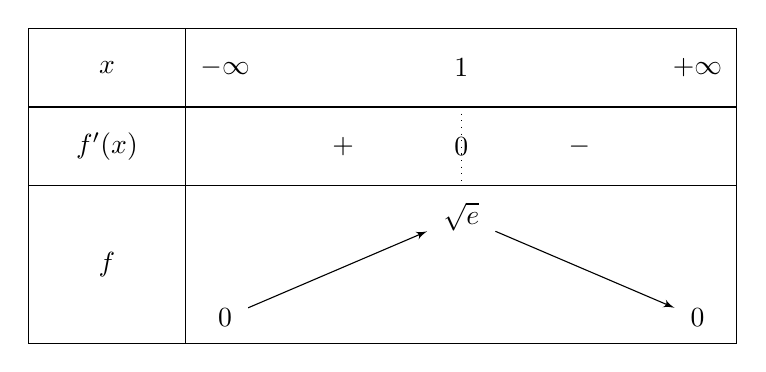
\begin{tikzpicture}[scale=1]
   \tkzTabInit{$x$ / 1 , $f'(x)$/1, $f$ / 2}{$-\infty$, $1$,$+\infty$}
   \tkzTabLine{, +, z, -,  }
   \tkzTabVar{-/$0$,+/$\sqrt{e}$,-/$0$}
\end{tikzpicture}
\end{center}

\item \(f'\) est dérivable sur \(\mathbb{R}\) comme produits de fonctions dérivables. Pour tout réel \(x\), 


\[ f^{\prime\prime}(x)=-4 \times \e^{-2x^2+4x-\frac{3}{2}} + (-4x+4)\times(-4x+4)\e^{-2x^2+4x-\frac{3}{2}}=(16x^2-32x+12)\e^{-2x^2+4x-\frac{3}{2}}.\]

\item \(f^{\prime\prime}(x)\) est du signe de \(16x^2-32x+12\). C'est un polynôme du second degré de discriminant \((-32)^2-4\times12\times16=256\). Ses racines sont \(\dfrac{1}{2}\) et \(\dfrac{3}{2}\). \(f\) est convexe sur \(\left[\dfrac{1}{2};\dfrac{3}{2}\right]\). La fonction admet des points d'inflexion aux abscisses \(\dfrac{1}{2}\) et \(\dfrac{3}{2}\).

\item Les équations des tangentes...
\begin{itemize}
\item A l'abscisse \(\dfrac{1}{2}\) : \(y=f'\left(\dfrac{1}{2}\right)\left(x-\dfrac{1}{2}\right)+f\left(\dfrac{1}{2}\right)\) soit \(y=2x\).
\item A l'abscisse \(\dfrac{3}{2}\) : \(y=f'\left(\dfrac{3}{2}\right)\left(x-\dfrac{3}{2}\right)+f\left(\dfrac{3}{2}\right)\) soit \(y=-2x+4\).
\end{itemize}

 \item Pour tout réel \(x\), 
\[f(2-x)=\e^{-2(2-x)^2+4(2-x)-\frac{3}{2}}=\e^{-2(4-4x+x^2)+8-4x-\frac{3}{2}}=\e^{-8+8x-2x^2-4x-\frac{3}{2}}=\e^{-2x^2+4x-\frac{3}{2}}=f(x).\]

La courbe de \(f\) est symétrique par rapport à la droite d'équation \(x=1\).

\item L'allure de la courbe \(\mathcal{C}_f\) dans un repère orthogonal est la suivante.

\begin{center}
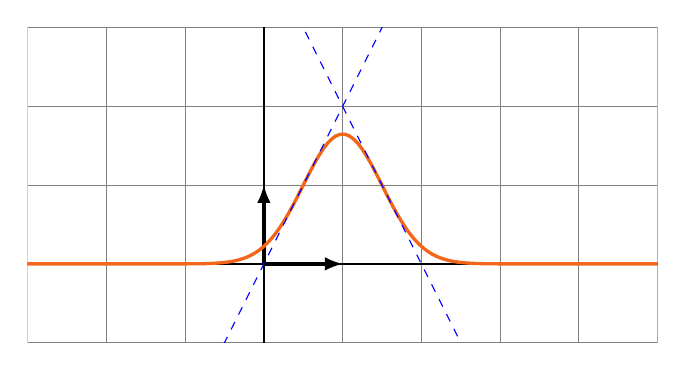
\begin{tikzpicture}[scale=1]
\clip (-3,-1) rectangle (5,3);
\draw [thin,gray] (-3,-4) grid (5,8);
\draw [thick] (-4,0)--(7,0);
\draw [thick] (0,-4) -- (0,6);
\draw [very thick,->,>=latex] (0,0)--(0,1);
\draw [very thick,->,>=latex] (0,0)--(1,0);
\draw [very thick, ocre,domain=-4:7,samples=200] plot (\x,{ exp(-2*\x*\x+4*\x-3/2) });
\draw [blue, dashed,domain=-4:5,samples=100] plot (\x,{2*\x});
\draw [blue, dashed,domain=-4:5,samples=100] plot (\x,{4-2*\x});
\end{tikzpicture}
\end{center}
\end{enumerate}
\end{solution}




\begin{exercise}[subtitle={(Centres étrangers 2022)}]
Soit $f$ la fonction définie sur l'intervalle $]0;+\infty[$ par
\[f(x)=x\ln(x)+1.\]
On note $\mathcal{C}_f$ sa courbe représentative dans un repère du plan.
\begin{enumerate}
\item Déterminer la limite de la fonction $f$ en 0 ainsi que sa limite en $+\infty$.
\item \begin{enumerate}
\item On admet que la fonction $f$ est dérivable sur $]0;+\infty[$ et on notera $f'$ sa fonction dérivée. Montrer que pour tout réel $x$ strictement positif,
\[f'(x)=1+\ln(x).\]
\item En déduire le tableau de variation de la fonction $f$ sur $]0;+\infty[$. On y fera figurer la valeur exacte de l'extremum de $f$ sur $]0;+\infty[$ et les limites.
\item Justifier que pour tout $x\in]0;1[$, $f(x)\in]0;1[$.
\end{enumerate}
\item \begin{enumerate} 
\item Déterminer une équation de la tangente $(T)$ à la courbe $\mathcal{C}_f$ au point d'abscisse 1.
\item Étudier la convexité de la fonction $f$ sur $]0;+\infty[$.
\item En déduire que pour tout réel $x$ strictement positif,
\[f(x)\geqslant x.\]\end{enumerate}
\item On définit la suite $(u_n)$ par son premier terme $u_0$ élément de l'intervalle $]0;1[$ et pour tout $n\in\mathbb{N}$,
\[u_{n+1}=f(u_n).\]
\begin{enumerate}
\item Démontrer par récurrence que pour tout entier naturel $n$, on a $0<u_n<1$.
\item Déduire de la question \textbf{3.c.} la croissance de la suite $(u_n)$.
\item En déduire que la suite $(u_n)$ est convergente.
\end{enumerate}
\end{enumerate}
\newpage
\end{exercise}

\begin{solution}\hspace{0pt}
\begin{enumerate}
\item Par croissances comparées, $\displaystyle\lim_{x\to 0^+}x\ln(x)=0$ et donc $\displaystyle\lim_{x \to 0^+}f(x)=1$. Par ailleurs, par produit, $\displaystyle\lim_{x\to +\infty}f(x)=+\infty$.
\item \begin{enumerate}
\item Pour tout réel $x>0$, $f'(x)=1 \times \ln(x)+x \times \dfrac{1}{x}=\ln(x)+1$.
\item Soit $x>0$, on a $\ln(x)+1 \geqslant 0$ si et seulement si $x \geqslant \e^{-1}$.
\begin{center}
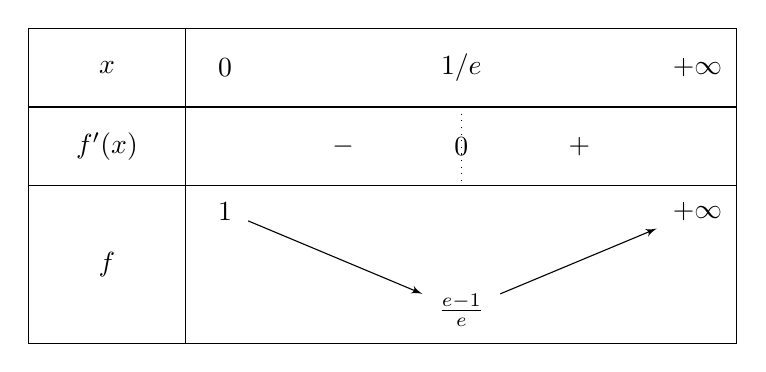
\begin{tikzpicture}[scale=1]
   \tkzTabInit{$x$ / 1 , $f'(x)$ / 1, $f$ / 2}{$0$, $1/e$, $+\infty$}
   \tkzTabLine{,-,z,+, }
   \tkzTabVar{+/$1$,-/$\frac{e-1}{e}$,+/$+\infty$}
\end{tikzpicture}
\end{center}
\item La fonction $f$ est strictement décroissante sur $]0;1[$. \\ Ainsi, si $0<x<1$, alors $1 > f(x) > \dfrac{e-1}{e}$ et en particulier, $f(x)\in]0;1[$.
\end{enumerate}
\item \begin{enumerate} 
\item La tangente $(T)$ a pour équation $y=f'(1)(x-1)+f(1)$ soit $y=1 x\times (x-1)+1$ et donc $y=x$.
\item $f$ est deux fois dérivable sur $]0;+\infty[$ et pour tout réel $x>0$, $f''(x)=\dfrac{1}{x}$. En particulier, $f''(x)>0$. $f$ est donc convexe sur $]0;+\infty [$.
\item Puisque $f$ est convexe sur $]0;+\infty[$, la courbe de $f$ est au-dessus de toutes ses tangentes sur cet intervalle. En particulier, elle se trouve au-dessus de la tangente $T$. Ainsi, pour tout réel $x$ strictement positif, $f(x)\geqslant x$.\end{enumerate}
\item 
\begin{enumerate}
\item Pour tout entier naturel $n$, on pose $P(n)$ : « $0<u_n<1$ ».
\begin{itemize}
\item On a bien $u_0 \in ]0;1($. $P(0)$ est donc vraie. 
\item Soit $n\in\mathbb{N}$. Supposons $P(n)$ vraie. On a donc $0<u_n<1$. Or, d'après la question \textbf{2.c.}, on a $f(u_n) \in ]0;1[$ soit $u_{n+1} \in ]0;1[$. $P(n+1)$ est donc vraie.
\item Par récurrence, $P(n)$ est vraie pour tout entier naturel $n$.
\end{itemize}
\item Pour tout entier naturel $n$, on a $f(u_n)\geqslant u_n$ d'après la question \textbf{3.c.}; Ainsi, pour tout entier naturel $n$, $u_{n+1}\geqslant u_n$. La suite $(u_n)$ est donc croissante.
\item La suite $(u_n)$ est croissante et majorée par 1. Elle est donc convergente.
\end{enumerate}
\end{enumerate}
\end{solution}





\begin{exercise}[subtitle={(Métropole 2021)}]

\paragraph{Partie A}

On donne ci-dessous, dans le plan rapporté à un repère orthonormé, la courbe représentant la\textbf{ fonction dérivée} $f'$ d'une fonction $f$ dérivable sur $\mathbb{R}$.

\begin{center}
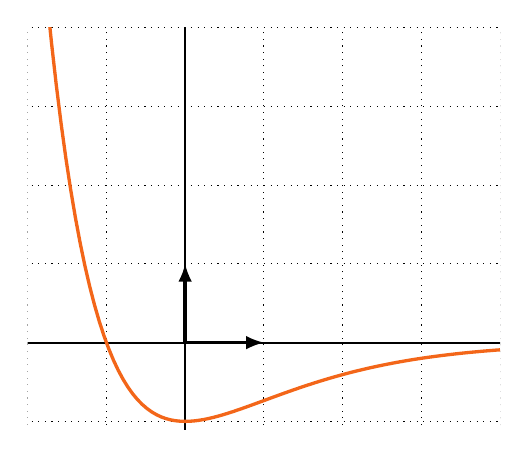
\begin{tikzpicture}[scale=1]
\clip (-2,-1.1) rectangle (4,4);
\draw [ thin, dotted] (-6,-4) grid (6,4);
\draw [thick] (-6,0)--(7,0);
\draw [thick] (0,-4) -- (0,5);
\draw [very thick,->,>=latex] (0,0)--(0,1);
\draw [very thick,->,>=latex] (0,0)--(1,0);
\draw [very thick, ocre,domain=-2:4,samples=100] plot (\x,{(-\x-1)*exp(-\x)});
\end{tikzpicture}
\end{center}

A l'aide de cette courbe, donner, en justifiant
\begin{enumerate}
\item Le sens de variations de la fonction $f$ sur $\mathbb{R}$ ;
\item La convexité de la fonction $f$ sur $\mathbb{R}$.
\end{enumerate}


\paragraph{Partie B}

On admet que la fonction $f$ mentionnée dans la Partie A est définie sur $\mathbb{R}$ par :
\[f(x)=(x+2)\e^{-x}\]
On note $\mathcal{C}$ la courbe représentative de $f$ dans un repère orthonormé $\Oij$.
On admet que la fonction $f$ est deux fois dérivable sur $\mathbb{R}$.
\begin{enumerate}
\item  Montrer que, pour tout nombre réel $x$,
\[f(x)=\dfrac{x}{\e^x}+\dfrac{2}{\e^x}.\]
En déduire la limite de $f$ en $+\infty$.\\
Justifier que la courbe $\mathcal{C}$ admet une asymptote que l'on précisera.\\
On admet que $\displaystyle\lim_{x \to - \infty}f(x)=-\infty$.
\item \begin{enumerate}
\item Montrer que, pour tout nombre réel $x$, $f'(x)=(-x-1)\e^{-x}$.
\item Étudier les variations sur $\mathbb{R}$ de la fonction $f$ et dresser son tableau de variations.
\item Montrer que l'équation $f(x) = 2$ admet une unique solution $\alpha$ sur l'intervalle $[-2; -1]$ dont on donnera une valeur approchée à $10^{-1}$ près.\end{enumerate}
\item Déterminer, pour tout nombre réel $x$, l'expression de $f''(x)$ et étudier la convexité de la fonction $f$. Que représente pour la courbe $\mathcal{C}$ son point $A$ d'abscisse 0 ?\end{enumerate}
\newpage
\end{exercise}

\begin{solution}

\paragraph{Partie A}


\begin{enumerate}
\item $f'$ semble positive sur $]-\infty ;-1]$ puis négative sur $[-1;+\infty[$. $f$ est donc croissante sur $]-\infty ; 1]$ et décroissante sur $[1;+\infty[$.
\item $f'$ semble décroissante sur $]-\infty;0]$ puis croissante sur $[0;+\infty[$. $f$ est donc concave sur $]-\infty ;0]$ puis convexe sur $[0;+\infty($.
\end{enumerate}


\paragraph{Partie B}

\begin{enumerate}
\item  Pour tout réel $x$, $f(x)=\dfrac{x+2}{\e^x}=\dfrac{x}{\e^x}+\dfrac{2}{\e^x}$. Or, par croissances comparées, $\displaystyle\lim_{x\to +\infty}\dfrac{x}{\e^x}=0$. Par ailleurs,  $\displaystyle\lim_{x\to +\infty}\dfrac{2}{\e^x}=0$. Ainsi,  $\displaystyle\lim_{x\to +\infty}f(x)=0$. La droite d'équation $y=0$ est asymptote à la courbe de $f$ en $+\infty$.
\item \begin{enumerate}
\item Pour tout réel $x$, $f'(x)=1 \times \e^{-x}+(x+2) \times (-\e^{-x})=(-1-x)\e^{-x}$.
\item Pour tout réel $x$, $f'(x)$ est du signe de $-1-x$.
\begin{center}
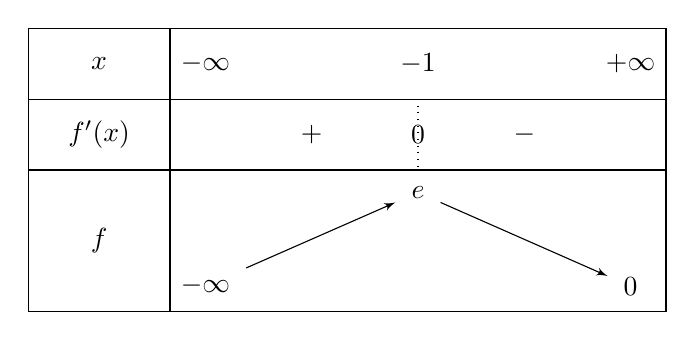
\begin{tikzpicture}[scale=0.9]
   \tkzTabInit{$x$ / 1 , $f'(x)$ / 1, $f$ / 2}{$-\infty$, $-1$, $+\infty$}
   \tkzTabLine{,+,z,-, }
   \tkzTabVar{-/$-\infty$,+/$e$,-/$0$}
\end{tikzpicture}
\end{center}
\item $f$ est continue sur $[-2;-1]$. De plus, $f(-2)=0$ et $f(-1)=e>2$. D'après le théorème des valeurs intermédiaires, l'équation $f(x) = 2$ admet une solution sur l'intervalle $[-2; -1]$. De plus, la fonction $f$ étant strictement croissante sur cet intervalle, cette solution est unique. A l'aide de la calculatrice, on trouve $\alpha \simeq -1.59$.\end{enumerate}
\item Pour tout réel $x$, $f''(x)=-1\e^{-x}+(-1-x) \times(-\e^{-x})=x\e^{-x}$. Ainsi, $f''(x)$ est du signe de $x$. $f$ est donc concave sur $]-\infty ;0]$ puis convexe sur $[0;+\infty($. Le point d'abscisse 0 de la courbe $\mathcal{C}$ est un point d'inflexion de la courbe.\end{enumerate}

\end{solution}



\begin{exercise}[subtitle={(Sujet zéro 2021)}]

Sur le graphique ci-dessous, on a représenté dans un repère orthonormé :
\begin{itemize}
\item la courbe représentative $C_f$ d'une fonction $f$ définie et dérivable sur $]0 ; +\infty[$ ;
\item la tangente $T_A$ à la courbe $C_f$ au point $A$ de coordonnées $\left(\frac{1}{e}\,;\,e\right)$ ;
\item la tangente $T_B$ à la courbe $C_f$ au point $B$ de coordonnées $\left(1\,;\,2\right)$.\end{itemize}
La droite $T_A$ est parallèle à l'axe des abscisses. La droite $T_B$ coupe l'axe des abscisses au point de coordonnées $(3 ; 0)$ et l'axe des ordonnées au point de coordonnées $(0 ; 3)$.

\begin{center}
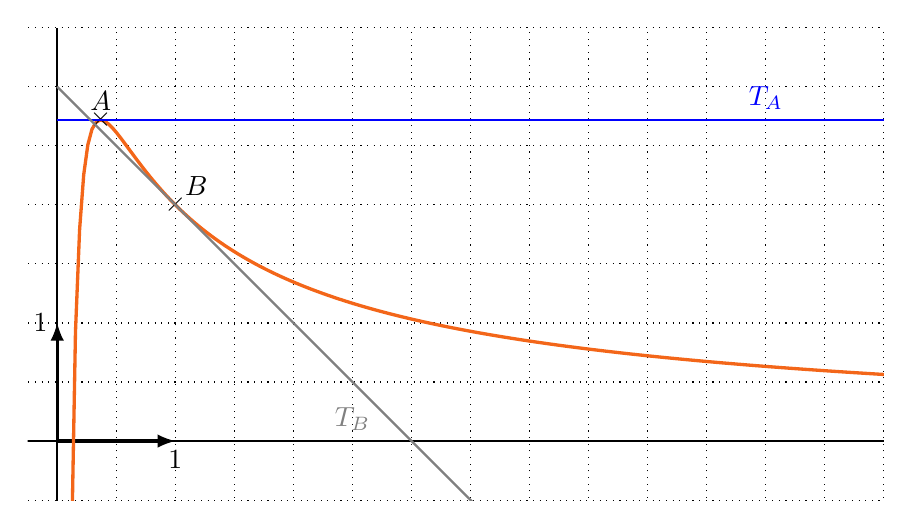
\begin{tikzpicture}[scale=0.75]
\clip (-0.5,-1) rectangle (14,7);
\draw [ thin, dotted] (-6,-4) grid (14,7);
\draw [thick] (-6,0)--(14,0);
\draw [thick] (0,-4) -- (0,7);
\draw [very thick,->,>=latex] (0,0)--(0,2);
\draw [very thick,->,>=latex] (0,0)--(2,0);
\draw (2,0) node [below] {1};
\draw (0,2) node [left] {1};
\draw [very thick, ocre,domain=0.1:14,samples=200] plot (\x,{2*(2+ln(\x/2))/(\x/2)});
\draw (2/2.718,2*2.718) node {$\times$} node[above] {$A$};
\draw (2,4) node {$\times$} node[above right] {$B$};
\draw [thick, blue,domain=0:14,samples=200] plot (\x,{2*2.718});
\draw [thick, gray,domain=0:14,samples=200] plot (\x,{6-\x});
\draw [thick, blue] (12,2*2.718) node[above] {$T_A$};
\draw [thick, gray] (5,0) node[above] {$T_B$};
\end{tikzpicture}
\end{center}

\paragraph{Partie A}

\begin{enumerate}
\item Déterminer graphiquement les valeurs de $f'\left(\dfrac{1}{e}\right)$ et $f'(1)$.
\item En déduire une équation de la droite $T_B$.
\end{enumerate}

\paragraph{Partie B}

On suppose maintenant que la fonction $f$ est définie pour tout réel $x \in ]0;+\infty[$ par
\[f(x)=\dfrac{2+\ln(x)}{x}.\]
\begin{enumerate}
\item Par le calcul, montrer que la courbe $C_f$ passe par les points $A$ et $B$ et coupe l'axe des abscisses en un unique point que l'on précisera.
\item Déterminer la limite de $f(x)$ quand $x$ tend vers 0 par valeurs supérieures et la limite de $f(x)$ quand $x$ tend vers $+\infty$.
\item Montrer que pour tout $x>0$
\[f'(x)=\dfrac{-1-\ln(x)}{x^2}.\]
\item Dresser le tableau de variations de $f$ sur $]0;+\infty [$.
\item On note $f''$ la dérivée seconde de $f$. 
\begin{enumerate}
\item Montrer que pour tout réel $x>0$,
\[f''(x)=\dfrac{1+2\ln(x)}{x^3}.\]
\item Déterminer le plus grand intervalle sur lequel $f$ est convexe.
\end{enumerate}
\end{enumerate}

\end{exercise}


\begin{solution}\hspace{0pt}


\paragraph{Partie A}

\begin{enumerate}
\item $f'\left(\dfrac{1}{e}\right)$ est le coefficient directeur de la tangente à la courbe de $f$ au point d'abscisse $\dfrac{1}{e}$, c'est-à-dire $A$. On a alors $f'\left(\dfrac{1}{e}\right)=0$. Par ailleurs, $f'(1)=-1$.
\item La tangente $T_B$ a pour coefficient directeur $-1$ et pour ordonnée à l'origine 3. Son équation réduite est donc $y=-x+3$.
\end{enumerate}

\paragraph{Partie B}

\begin{enumerate}
\item On a $f\left(\dfrac{1}{e}\right)=\dfrac{2+\ln(\e^{-1})}{\frac{1}{e}}=(2-1)e=e$ et $f(1)=\dfrac{2+\ln(1)}{1}=2$. La courbe $C_f$ passe par les points $A$ et $B$. De plus, pour $x>0$, $f(x)=0$ si et seulement si $2+\ln(x)=0$ soit $x=\e^{-2}$. La courbe $C_f$ coupe l'axe des abscisses au point de coordonnées $(\e^{-2};0)$.
\item En utilisant les règles de calcul sur les limites, on a que $\displaystyle\lim_{x\to 0^+}f(x)=-\infty$. Par ailleurs, pour tout réel $x>0$, $f(x)=\dfrac{2}{x}+\dfrac{\ln(x)}{x}$. Or, $\displaystyle\lim_{x\to+\infty}\dfrac{2}{x}=0$ et, par croissance comparées, $\displaystyle\lim_{x\to+\infty}\dfrac{\ln(x)}{x}=0$ Ainsi, $\displaystyle\lim_{x\to+\infty}f(x)=0$.
\item Pour tout $x>0$, $f'(x)=\dfrac{\frac{1}{x} \times 1 - (2+\ln(x))\times 1}{x^2}=\dfrac{1-2-\ln(x)}{x^2}=\dfrac{-1-\ln(x)}{x^2}$.

\item Soit $x>0$. Alors $-1-\ln(x)\geqslant 0$ si et seulement si $\ln(x) \leqslant -1$ soit $x\leqslant \e^{-1}$.
\begin{center}
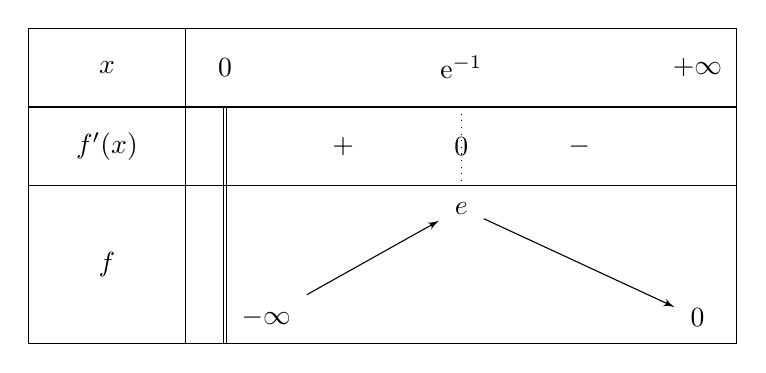
\begin{tikzpicture}[scale=1]
   \tkzTabInit{$x$ / 1 , $f'(x)$ / 1, $f$ / 2}{$0$, $\e^{-1}$, $+\infty$}
   \tkzTabLine{d,+,z,-, }
   \tkzTabVar{D-/$-\infty$,+/$e$,-/$0$}
\end{tikzpicture}
\end{center}

\item 
\begin{enumerate}
\item Pour tout réel $x>0$, $f''(x)= \dfrac{-\frac{1}{x} \times x^2 -(-1-\ln(x))2x}{x^4}=\dfrac{x(-1+2+2\ln(x))}{x^4}=\dfrac{1+2\ln(x)}{x^4}$.
\item Soit $x>0$. On a $f''(x) \geqslant 0$ si et seulement si $1+2\ln(x) \geqslant 0$ soit $\ln(x)\geqslant -\dfrac{1}{2}$ et $x\geqslant \e^{-1/2}$. $f$ est convexe sur $[\e^{-1/2};+\infty($.
\end{enumerate}
\end{enumerate}

\end{solution}





\chapter{Corrigés}


\printsolutions[headings={false} ]




\end{document}